\documentclass[12pt, letterpaper] 
%\documentclass[12pt, letterpaper, doublespace]{article} 
\usepackage[top=1in, bottom=1in, left=1in, right=1in]{geometry} 
\usepackage{setspace}
\doublespacing
\usepackage{amsmath} 
\usepackage{amsfonts} 
\usepackage{natbib}
\usepackage{mathtools} 
\usepackage{ragged2e} % for text justification
\usepackage{adjustbox} 
\usepackage{amssymb}
%\usepackage[capposition=top]{floatrow} 
\usepackage{fullpage} 
\usepackage{listings}
\usepackage{dcolumn} 
\usepackage{bigstrut} 
\usepackage{float} 
\usepackage{enumitem} 
\usepackage{url}
\usepackage[clockwise]{rotating} 
\usepackage{rotfloat} 
\usepackage{rotate} 
\usepackage{rotating}
\usepackage{pdflscape} 
\usepackage[labelfont=bf]{caption} 
\usepackage{graphicx} 
\usepackage{array}
\usepackage{booktabs} 
\usepackage[flushleft]{threeparttable} 
\usepackage{threeparttablex} 
% Lets threeparttable work with longtable 
\usepackage[outdir=graphics/]{epstopdf} 
\usepackage{graphics}
\usepackage{longtable} 
\usepackage[width=.95\textwidth]{caption}
\usepackage{changepage} 
% for the adjustwidth environment
%\let\oldtabular\tabular 
%\renewcommand{\tabular}{\footnotesize\oldtabular}
\newcommand\Fontvi{\fontsize{8}{7.2}\selectfont}
%\newcolumntype{L}{>{\centering\arraybackslash}m{3cm}}
\newcolumntype{L}[1]{>{\raggedright\let\newline\\\arraybackslash\hspace{0pt}}b{#1}}
\newcolumntype{C}[1]{>{\centering\let\newline\\\arraybackslash\hspace{0pt}}b{#1}}
\newcolumntype{R}[1]{>{\raggedleft\let\newline\\\arraybackslash\hspace{0pt}}b{#1}}

%\setlength{\textwidth}{150mm} 

%\linespread{1} 
%\linespread{1.7}

\bibpunct{(}{)}{;}{a}{,}{,}

\begin{document} 

\title{Accounting Policy Similarity and Active vs. Passive Institutional Investors}
\author{Reginald Edwards\footnote{Ross School of Business, University of Michigan
(\texttt{reggie@umich.edu}). I would like to thank my dissertation committee chairs Raffi Indjejikian and Venky Nagar and members Allison Earl and Robert F. Dittmar. I am also grateful for the advice and comments of Ryan Ball, Greg Miller, Cathy Shakespeare, Christopher Williams, and Reuven Lehavy, as well as workshop participants at the University of Michigan. I appreciate the financial support of the Ross Doctoral Fellowship, the Paton Accounting Fellowship, and the University of Michigan Rackham Merit Fellowship.}} 
\date{Aprile 2018}

\maketitle 
\begin{abstract} 
I examine the differential effects of accounting comparability on investment by active and passive institutional investors. I develop a novel measure of accounting comparability based on the textual disclosure of firms' accounting policies from their annual reports and find that, among firms with less comparable accounting, investment by active institutions is higher than that of passive institutional investors. This suggests that these investors have a real or perceived information advantage in investing in firms with less comparable accounting. To establish causality, I use a difference-in-differences approach that relies on the plausibly exogenous introduction of an accounting rule change, which is likely to decrease comparability, and the rule's subsequent reversal. My paper offers novel evidence on an under-explored relation between accounting comparability and investor preferences.
\end{abstract}

\newpage 

\section{Introduction}\label{introduction} 
% Introduction for non-accounting researchers
%
% Describe the accounting information environment.
% Describe investors, who they are, and what we know about their behavior, why they're important etc.
% What is "comparability"?

Prior empirical studies have assumed that institutional investors uniformly prefer firms with more comparable accounting \citep{defondetal2011, fangetal2015, kimetal2016}. However, theoretical models predict that investors' preferences for information from firms depends on the degree of their private information \citep[see][]{easleyohara2004}. In this study, I attempt to determine if investors who take a more active approach or a more passive approach to selecting stocks prefer firms with accounting reports that I identify as more or less comparable to their peer firms. 
I first demonstrate that managers' discretion over implementing accounting rules influences the degree to which their accounting reports are comparable to peer firms. Using this finding, I identify an accounting rule change that reduced managers' discretion in recognizing revenue and its subsequent reversal  to identify causally the differential impact of accounting comparability on the behavior of active and passive investors. To address my research question, I develop and validate a novel proxy for the comparability of firms' financial statements.  And, appealing to the plausibly exogenous nature of the shock to comparability induced by the accounting rules,  I provide evidence that investors who are more likely to trade based on superior private information prefer less comparabale accounting than investors who are more likely to trade based on public information.

The Financial Accounting Standards Board \citep{fasb2010} lists comparability of accounting reports as a potentially enhancing characteristic of financial information. The FASB view is that, along with verifiability, timeliness, and understandability, comparability enhances information that is already relevant and accurate.\footnote{In the language of the FASB, accurate information is that which is ``faithfully represented''--that is, ``complete, neutral, and free from error''; relevant information is that which lends itself to being used to forecast outcomes or confirm past outcomes.} Comparability of financial accounting statements implies that similar economic events should map to similar accounting reports and dissimilar events to dissimilar reports. For this, a necessary condition is the consistent calculation of revenues and expenses and liabilities and assets. I define accounting comparability as the similarity of accounting choices among firms and measure it accordingly. Commonly cited examples of choices that can alter comparability are the treatment of inventory (last-in, first-out versus first-in, first-out), the classification of leases as operating or capital leases, and the more all-encompassing choice of US Generally Accepted Accounting Principles or International Financial Reporting Standards. The common thread is that to the extent that accounting rules allow discretion by managers, different choices by managers may lead to higher or lower levels of comparability across firms. Below I describe two settings in which the level of discretion afforded to managers under the accounting rules shifted. These settings will be useful in establishing a causal link between accounting comparability and investor ownership.

Effective as of the end of 1998, accounting standard setters created Statement of Position 97-2 (SOP 97-2), to constrain the discretion of managers in firms that engage in multiple-element software products and services. These rules governed the recognition of revenue for the sale of products that were bundled with services for installation, updates, and ongoing customer support. The standard was set in response to perceived aggressive revenue recognition by software firms. Due to the complex nature of contracts for then new bundled software and services stretching over many periods, managers had significant leeway to use estimates and assumptions when assigning revenue generated from these sales. As a result of SOP 97-2 firms that sold products or services with a significant software-based component were required to adhere to a more uniform set of revenue recognition principles. However, provisions of this rule were later removed by an accounting standard update in 2009.\footnote{FASB Accounting Standards Update 2009-13 and 2009-14, effective June 15 2010.} This rule change limited the scope of SOP 97-2 and returned to managers of firms who sold products and services with a mix of software and non-software components (i.e., multiple element arrangements) a high level of discretion. In this paper I argue that both rule changes represent a plausibly exogenous shock to the level of comparability of firms' financial statements and I examine the differential impact on active and passive institutional investors. To do so, I must define and construct a measure of accounting comparability at the individual firm-level.

I compare the textual description of firms' accounting policies from their annual reports (Form 10-Ks) to the descriptions disclosed by their peer firms to create a measure of accounting comparability. These disclosures capture the major accounting choices firms make, which influence the ability of financial statement users to compare accounting information across firms at a given point in time and over time for a given firm.

% Why do we care about comparability's affect on institutional ownership? 
Certain large institutional investors trade primarily on widely available public information \citep{busheegoodman2007}--these I label passive investors. I argue that these investors prefer accounting figures that are more comparable across firms. There are three reasons that this may hold. The first is that simple accounting-based valuation tools, such as ratio analysis and comparisons of multiples, are more successful when establishing a comparable peer firm is easier \citep{bhojrajlee2002, youngzeng2015, leeetal2015}. Second, as \cite{bradshawetal2009} document, analyst forecasts are more useful in more comparable industries--another reason investors may prefer comparable accounting. Third, A more comparable accounting system makes it harder for a single manager to hide bad news from investors \citep{kimetal2016}.

In contrast, for active investors--those who trade on perceived comparative information advantages--the opposite case may hold. There is theoretical and empirical evidence that sophisticated investors may prefer firms with a more opaque information environment. This opacity may allow these investors to profit from superior information processing capabilities \citep{kimverrecchia1994} or privately acquired information \citep{maffett2012}.

% Discuss results
My OLS results are consistent with this intuition. To provide evidence on the direction of causality, I exploit the accounting rule changes in SOP 97-2 and ASU 2009-13 that present plausibly exogenous \emph{opposing} shocks to the comparability of a subset of firms. Using a difference-in-differences (DD) specification, I find that decreased comparability causes higher investment by active investors relative to passive investors, and vice-versa.

The rest of the paper is organized as follows. Section \ref{lit-review} reviews relevant studies and describes my empirical design, identification strategy, and proxy for earnings comparability. Section \ref{data} describes data sources and presents descriptive statistics. Sections \ref{results} presents empirical results. Section \ref{conclusion} concludes.

\section{Motivation and Background}\label{lit-review} 
\subsection{Two Quasi-Natural Experiments: SOP 97-2 and ASU 2009-13}
%To estimate the causal impact of accounting comparability on institutional investor ownership, I use the adoption of an accounting rule that increased the comparability of firms' financial statements and its subsequent reversal.
% SOP 97-2
The American Institute of Certified Public Accountants' (AICPA's) Statement of Position 97-2 (SOP 97-2) reduced the amount of discretion managers of affected firms had with respect to one aspect of revenue recognition. 
% Why were they passed? (Plausible exogeneity to your outcome variable)
% What firms do they affect and over what time periods?
% What do the rules specify?
SOP 97-2 was put forth to curtail revenue recognition practices that were perceived to be overly aggressive. Specifically, firms that sold software were able to shift revenue across reporting periods. This is because software-based products began to shift from a good to more of a service. Software updates and support were bundled into the initial price but would be delivered over future months and, increasingly, years. This growing mismatch of revenues and expenses could allow firms to prematurely allocate a portion of the selling price to revenue. SOP 97-2 required a strict precedent, known as vendor specific objective evidence (VSOE), for recognizing revenue from these multiple element arrangements. The fair-value-like requirement of VSOE meant that firms needed a long history of standalone pricing for each element in a multielement arrangement \citep{cfo2008}. Without this evidence, firms would have to delay the recognition of all revenues until all services have been delivered.

% EITF 09-3
% Why were they passed? (Plausible exogeneity to your outcome variable)
% What firms do they affect and over what time periods?
% What do the rules specify?
Over time, as more products began to incorporate software components, the range of products and services covered by SOP 97-2 grew beyond that initially intended by standard setters. Subsequently, FASB introduced an updated standard to reduce the scope of SOP 97-2. Known as Accounting Standards Update (ASU) 2009-13, this rule limited SOP 97-2 to pure software transactions and allowed managers to make use of estimates when allocating the price of longer term contracts to deliver bundled software services.

The limited discretion allowed under SOP 97-2 may have increased the comparability of these firms financial statements to each other by forcing similar economic transactions to appear similar.\footnote{It is possible the comparability of reported income statement numbers decreased by forcing dissimilar economic transactions to appear similar. For my setting it is only necessary that companies \emph{appear} to have more similar accounting, which would generate a disincentive for investors to exert effort collecting and analyzing information. A simple example illustrates this point. Consider two firms, Firm 1 and Firm 2, that have agreed to provide \$100 in service over the next four years. Firm 1 will provide an equal value of the service over each period (i.e. \$25 in each year). Firm 2 will provide \$25 worth of service in year 1 and \$75 worth in year 4. SOP 97-2 would require both firms to recognize \$0 in revenue for the first three years and \$100 in the fourth. In the presence of the accounting rule, managers would be barred from using their judgment in deciding when to recognize each amount of revenue. These transactions, with markedly different underlying economics, would appear similar. However, managers have extensive leeway to widely disclose non-GAAP figures in such cases. They have much less incentive and leeway to discuss these effects in the Significant Accounting Policies section of the 10-K, which is the focal point at which I measure comparability.} 
I view this case as likely and prior research has documented a pervasive pattern of increased discretion given to managers (e.g., \cite{dechowskinner2000}, \cite{beneish2001}, \cite{hribarjenkins2004}, \cite{beattyetal2002}, \cite{ayersetal2006}) leading to lower quality financial statements. Empirically, this is the association I document between comparability and the introduction of SOP 97-2.\footnote{Anectdotally, Boeing has recently come under scrutiny for its atypical accounting for large upfront investments in developing airplanes and the extensive use of estimates in allocating the costs of the planes (\cite{ostrower2014}). The accounting rules permit this level of discretion by Boeing's managers, but other manufacturers in the same industry allocate the majority of the cost upfront. This is a typical real world example of the mechanism by which I view more discretion as leading to lower comparability.} At the same time, this rule increased the potential gains to superior private information of firms. Investors with the ability or an endowment of more precise information as to the nature of the underlying transactions would thus benefit. 

Through similar reasoning, the reversal of parts of SOP 97-2 by ASU 2009-13 allows me to identify the effect of decreasing comparability on the ratio of active-to-passive institutional investor ownership.

% EITF 09-3
\subsection{Defining and Measuring Financial Statement Comparability} \label{comparability}
Financial statement analysis textbooks \citep[see]{healypalepu2007, kolleretal2005} generally advise users of financial statements to begin an accounting-based comparison of peer firms by noting discrepancies in the calculations and assumptions used to generate balance sheet and income statement numbers. This is because the extent to which the accounting numbers of two firms can be compared and how likely their future perfomance is to covary depend on the accounting choices used to map economic reality to reported numbers. 

As required by US GAAP, firms discuss the details of these calculations and assumptions in their annual reports.
Therefore, my starting point for the measurement of accounting comparability is the ``Summary of Significant Accounting Policies'' from firms' annual report, the standard location of these disclosures. These disclosures are nested within the ``Notes to the Financial Statements'' section, after the audited financial statements. 

I extract the ``Summary of Significant Accounting Policies''  section from the financial statements computationally. I then use a document similarity algorithm to compare the text in this section of each firm reporting in a given fiscal year to each other firm in that fiscal year. I explain in more detail the exact procedure in the Appendix. In short, each selection of text is viewed as a collection of word ``tokens'' and the frequency of each token in each document is counted. Two documents are then compared based on the number of words they have in common and how often they contain each of those words. The result is that documents that contain many of the same words will have a high similarity score and two selections of text that have do not share many words will have a very low similarity score.\footnote{One of the first papers in finance and accounting to use this approach to compare firms' disclosures was \cite{hobergetal2014}, which compared the product discreptions from the ``Item 1. Business'' sections across firms' annual reports.}

I use the accounting policy descriptions to measure accounting comparability because they directly address the firm's treatment of economic transactions in the financial statements. By comparing these disclosures to peer firms, the measure attempts to capture differences in accounting that are not due to merely differences in firm structure. In regression analyses control variables help to further address this concern.

Financial reports are a mix of quantitative figures (net income, assets, cash flows etc.) and textual disclosures, which are intended to help financial statement consumers understand the process by which the figures were generated. These disclosures cover many aspects of firms' operational environment and potential future risks, the Summary of Significant Accounting Policies section of the notes to the financial statements directly addresses the assumptions and procedures used to map the firm's economic reality to its accounting figures. While many different accounting treatments may lead a firm to calculate net income as \$100, the more the firm discloses about the underlying process the better investors will be able to assess performance and assign value. Essentially, I view earnings (and other accounting figures) computed in similar ways as comparable.

My input-based measure of accounting comparability differs from the output-based methods of \cite{bhojrajlee2002} and \cite{defrancoetal2011}, who use a regression-based approach to estimate mappings from returns to earnings for a focal firm and apply these to a target firm. Comparability in these studies is measured as the accuracy of these projected earnings. Similar methods have been used in recent work to link accounting comparability to peer earnings restatements (\cite{campbellyeung2016}), the valuation of seasoned equity offerings (\cite{shaneetal2014}), and expected crash risk (\cite{kimetal2016}). I add to this growing literature by proposing a measure of comparability less sensitive to the estimation problems of these measures. Specifically, my measure of comparability does not require more than two years of financial reports, nor does it rely on a statistical relations between earnings and returns that  are likely to be very weak.

Financial statement comparability is a function of firms' business environments (economic reality), the accounting rules, and the managerial discretion allowed under the accounting rules. I attempt to hold the first two inputs constant and appeal to plausibly exogenous variation in the latter input to establish a causal link between comparability and investor behavior.

\subsection{Active vs. Passive Institutional Investors} 
Institutional investors--mutual funds, pensions, endowments, hedge funds, and banks--today own an aggregate of 80\% of publicly traded shares and owing to their central role in the capital markets,institutions have been a focus of research in finance and accounting for at least three decades. Studies have found that institutions prefer stocks with high volatility and low transactions costs (\cite{falkenstein1996}) and firms that are larger, more liquid, and have had recently depressed stock prices (\cite{gompersmetrick2001}). 

According to theoretical work of \cite{merton1987}, firms are likely to benefit from an increased investor base and recent surveys of institutional investors by the Organization for Economic Cooperation and Development (\cite{oecd2014}) indicate that this is a primary concern for managers.\footnote{In addition to the presence of institutional investors the type of institutions (e.g., long-term or short-term) can have a profound impact on managers' incentives. The OECD contend that attracting long-term institutional investors is an active and worthwhile goal for policymakers because infrastructure investments may be appealing to large institutions because they tend to take a long-term investment horizon (\cite{oecd2014}).} Corroborating this, empirical studies (\cite{lehavysloan2008}) have documented the benefits of increased ownership of firms' shares by institutional investors (e.g. mutual funds, hedge funds, pensions and endowments). Therefore it is important to understand the drivers of investment by different types of institutions. \footnote{Many of the empirical studies in accounting and finance that have combined to map the preferences of institutional investors broadly belong to one of two research streams--those that find drivers of institutional investor demand and those studies that examine the impact of investment by institutions. Real and financial outcomes that have been previously studied are payout policy (\cite{grinsteinmichaely2005}), corporate governance (\cite{chungzhang2011}), operating performance and capital expenditure (\cite{ferreiramatos2008}), transparency surrounding corporate pension plans (\cite{eatonetal2014}), the public-to-private takeover premium (\cite{bajo2013}), and stock return volatility (\cite{busheenoe2000})}

Two of the earliest studies to address how features of the financial reporting environment influence institutional investor ownership are \cite{healyetal1999} and \cite{busheenoe2000}. Both papers focus on disclosure quality as a driver of investor demand. Both papers also find that institutions invest more in firms with higher quality disclosure, as proxied by equity research analysts' subjective ratings of disclosure. My work adds to these prior studies by including financial statement comparability as another feature of the reporting environment that affects investor demand. However, I do not address the economic impacts of these institutional preferences. My focus is financial reporting quality as a driver of institutional ownership rather than the outcomes associated with the latter.\footnote{Economic outcomes of institutional ownership have been studied in \cite{lehavysloan2008}, \cite{grinsteinmichaely2005}), \cite{chungzhang2011}, \cite{ferreiramatos2008}, \cite{eatonetal2014}, \cite{bajo2013}, \cite{busheenoe2000}, among others. See Section \ref{lit-review} for a discussion of this literature. }

The view that institutions prefer firms with more comparable accounting is directly supported by \cite{defondetal2011}, who examine the link between cross-border investment and uniformity of accounting policy in the EU around adoption of IFRS. The authors find that mandatory IFRS adoption increased ownership by mutual funds of firms outside of their home countries when adoption in the target country was (a) highly credible; \emph{and} (b) led to a large increase in uniformity. \cite{defondetal2011} however, do not find that mandatory IFRS adoption increased mutual fund ownership in firms in their home countries. A potential explanation for this non-result is that an increase in uniformity of accounting standards associated with IFRS did not make firms' accounting information significantly more comparable within countries to alter the investment strategies of institutions. This view is consistent with the evidence in \cite{yipyoung2012} and \cite{cascinogassen2015}, which show no strong increase in country comparability around the adoption of IFRS in EU countries.

Another possible explanation for the non-result of \cite{defondetal2011} is that some domestic mutual funds enjoy a comparative advantage in information processing among their home-country firms. Thus, on net these funds would not stand to benefit from any increase in comparability among the home-country firms. Thus my primary hypothesis is stated as follows:

\begin{adjustwidth}{1cm}{} 
\textbf{Hypothesis 1} \emph{The relative percentage of shares held by active institutional investors to passive investors is decreasing in the degree of earnings comparability.} 
\end{adjustwidth}

\section{Data Sources, Variable Definitions, and Descriptive Statistics} \label{data} 
Company accounting data are from Compustat, stock price and returns data are from CRSP, analyst forecast and coverage data from IBES, and data on institutional holdings are from Thomson-Reuters' 13-F database. My data span all stocks listed on the NYSE, NASDAQ, or American Stock Exchange (AMEX) and all industries over the years 1994 to 2015. I define institutional ownership for each firm in each year as the ratio of shares held by institutions to the total shares outstanding. I limit my sample to December fiscal-year-end firms. My final sample consists of 41,159 firm-year observations. Table \ref{ior-mve-summary} contains summary statistics of the institutional investor holdings for 1980-2015, raw and unclassified in terms of active or passive investors for comparisons with prior studies. Over the entire time period for which data are available, institutional investors held over 41\% of shares in firms.\footnote{In recent years, this number is approximately 80\%.}

Table \ref{ior-mve-summary} also shows a decomposition of institutional ownership percentage by market value of equity. For comparison, I present statistics for the sample used in this study alongside the time period considered in \cite{grinsteinmichaely2005}'s study on institutional holdings and payout policy. Their study only covers the period up to 1996 and has very different selection process based on the data needs for their analysis, yet the patterns of institutional ownership by market capitalization are qualitatively similar. 

My classification for active and passive investors is derived from the institutional investor classification data provided by Brian Bushee\footnote{http://acct.wharton.upenn.edu/faculty/bushee/IIclass.html}. These classifications in turn are derived from and improvements on Thomson Reuters' classification scheme. I classify active investors as investment companies, independent investment advisors, corporate (private) pension funds, public pension funds, and university and foundation endowments. I classify passive investors as banks and insurance companies. My primary outcome variable is the ratio of dollars held by active investors to that of passive investors, which I label $PCT\text{-}ACTIVE$. My secondary outcome variable is the ratio of the number of active investors to passive investors, $NUM\text{-}ACTIVE$. The bottom panel of Table \ref{summary-stats} contains summary statistics for these variables, which indicate that the majority of firms (a 95\% confidence interval) have a share of active-to-passive investment, herein defined, between 60\% and 100\%.

To compute my proxy for accounting comparability, I retrieve all 10-K filings from the Securities and Exchange Commission's EDGAR database of company filings. I extract the ``Summary of Significant Accounting Policies'' section of the footnotes using textual analysis algorithms I implement in the Python programming language. Details on the mathematical basis for the construction of the measure are given in the appendix. For each firm I compute the similarity of its accounting policy disclosures to that of firms in the same industry (2-digit SIC code) in the same year. I then average the comparability score for each firm-year and denote this value as $COMP$. The bottom panel of Table \ref{summary-stats} contains summary statistics for my comparability measure. The percentile values of $COMP$ indicate sufficient variation, but by themselves lack a clear interpretation. Therefore I perform a univariate regression with $COMP$ as the dependent variable and each of my subsequent control variables. This provides an empirical explanation of the sources of variation in comparability. Reported in Table \ref{cossim-uni}, I find that $COMP$ is negatively associated with measures that largely capture firm complexity--age, size, and payout and leverage structure. Comparability is positively associated with asset tangibility and liquidity and is not statistically associated with capital market related factors.

\section{Accounting Policy Similarity Measurement}
\subsection{Definition}
My accounting comparability measure is a cosine similarity measure of the changes in words firms use to describe  their significant accounting policies in the footnotes to their annual reports. I compare these disclosures to that of peer firms. My presumption is that these disclosures from managers represent a meaningful source of information, which investors can use to compare numerical accounting figures across firms. This is in-keeping with the original Accounting Principles Board pronouncement around such information:

\begin{quote}
\footnotesize
Applying generally accepted accounting principles requires that judgment be exercised as to the relative appropriateness of acceptable alternative principles and methods of application in specific circumstances of diverse and complex economic activities. ...

The accounting policies of a reporting entity are the specific accounting principles and the methods of applying those principles that are judged by the management of the entity to be the most appropriate in the circumstances to present fairly financial position, cash flows, and results of operations in accordance with generally accepted accounting principles and that, accordingly, have been adopted for preparing the financial statements.

The accounting policies adopted by a reporting entity can affect significantly the presentation of its financial position, cash flows, and results of operations. Accordingly, \textbf{the usefulness of financial statements for purposes of making economic decisions about the reporting entity depends significantly upon the user's understanding of the accounting policies followed by the entity.}
\end{quote}
(APB 22, emphasis added)

The construction of comparability, $COMP$,  between two sets of accounting policy disclosures involves three components. First, denote  the set of all words occurring in the ``Summary of Significant Accounting Policies'' descriptions in a year is $\Omega_t$. We measure a  scalar, $J_t \equiv \vert\vert \Omega_t \vert\vert$, that is, the number of unique words used in  the descriptions of both firms. For each firm $i$ in year  $t$, an ordered binary vector $W_{it}$ is constructed such that each element $W^{(j)}_{it}$ of  $W_{it}$ is one if and only if word $j$ occurs in the given firm's text in the given  year. Let $N_{it} \equiv W_{it}/\vert\vert W_{it} \vert\vert,$ the normalized vector of word  occurrences for each firm-year. For each year, construct a similar vector $U_t$ of size $J_t$ in  which each element $U^{(j)}_t$ is equal to the sum of the number of occurrences of each word $j$  among both sets of text. From this vector, compute a measure of the aggregate  change in text from year $t-1$ to year $t$ as the change in the number of times the word was used. Denote this aggregate word use change variable as  $D_{t-1,t}$. 

Formally,
\begin{equation}
D_{t-1,t} \equiv \bigg\vert\bigg\vert \sum_{j} (U_{j,t} - U_{j, t-1}) \bigg\vert\bigg\vert.
\end{equation}

The comparability of a firm in a year is constructed as
\begin{equation}
COMP_{it} \equiv \frac{W_{it}}{\vert\vert W_{it} \vert\vert} \cdot \frac{D_{it}}{\vert\vert D_{it} 
\vert\vert},
\end{equation}
which is the cosine of the angle between the firms' vectors of word occurrences and the aggregate word change vector.

In subsequent analysis I make use of a measure of a firm's \emph{self} comparability, 
\begin{equation}
COMP_{it} \equiv 1 - \frac{W_{it}}{\vert\vert W_{it} \vert\vert} \cdot \frac{W_{it}}{\vert\vert 
W_{it} \vert\vert},
\end{equation}

which attempt to measure the degree to which the firm is changing its own accounting policies from one year to the next. By construction,  the comparability measure is on the closed interval from zero to one. 

\subsection{Preprocessing}
% steps to download 10-K's. Discuss attrition, compustat matching
% steps to extract SAP, discuss attrition. Summary stats to show representativeness (ts, xs, industry)
% lemmatization and stemming
To more accurately analyze the 10-K sections I perform several preprocessing steps on the corpus. Specifically, I remove alphanumeric sequences, convert all words to lowercase, and perform stemming and lemmatization on each document.
Stemming is...
Lemmatization is...
These steps should reduce the amount of noise in the construction of accounting similarity.

% tf-idf weighting
% computation of pairwise cossim
% summary stats: n-gram analyses, time-series, cross-section, industry
The graphs below show the time series and cross-sectional distributions of these two measures. As expected, own-firm comparability tracks that of $COMP$ for each firm, but is almost always higher.


%Discuss Potential Selection Bias 
% Discuss Collinearity 
\subsection{Control Variables} 
For each observation I control for a variety of factors that may confound the relationship between active investor ownership and comparability. These are liquidity demands of institutions \citep{falkenstein1996, ferreiramatos2008, huang2009}, preferences by institutions for larger companies \citep{gompersmetrick2001} and dividend payers \citep{grinsteinmichaely2005}, and the age and leverage of constituent firms \citep{badrinathetal1996}. 

The control variables I include are the number of years the firm appears in Compustat ($AGE$), the ratio of monthly trading volume to number of shares outstanding ($TURNOVER$), the stock return over the preceding year ($RETURN$), the average daily stock price over the preceding year ($PRICE$), the natural logarithm of the book value of assets ($ASSETS$), the natural logarithm of market capitalization ($MVE$), the average bid-ask spread ($BASPREAD$), an indicator variable for whether or not the firm is in the S\&P 500 ($SP500$), the dividend yield ($DIV$), the ratio of the book value of total debt to assets ($LEVERAGE$), Tobin's $q$ ($Q$), calculated as in \cite{chungpruitt1994}, return on assets ($ROA$)--the ratio of net income to the book value of total assets, and the level of asset tangibility ($TANG$), calculated as in \cite{almeidacampello2007}. 

I include the number of equity research analysts who provide earnings forecasts for the firm ($NANALYSTS$), as a proxy for the quality of the information environment of the firm. Table \ref{summary-stats} shows summary statistics for these variables. These variables are very similar to those in \cite{chungzhang2011}, who use a similar set of control variables. Finally, I include the \emph{forward} price-to-earnings ratio ($PE$)--computed as the current period stock price divided by the one-year-ahead analyst consensus earnings forecast--as a measure of investors' performance expectations for the firm.

\section{Empirical Results}\label{results}
\subsection{Baseline Ordinary Least Squares Results}
For each firm in each fiscal year in my sample, I compute the comparability between that firm and all other firms in its industry (2-digit SIC). I then take the median over all industry peers as that firm's level of comparability. My dependent variable is the ratio of active-to-passive investors for each firm as of that firm's fiscal year-end date. In all subsequent regressions I lag my variable of interest, $COMP$, and all control variables. I also rank $COMP$ for each firm into deciles by year.

\subsubsection{Regression of Levels of Active-to-Passive Ownership Ratio} 
To assess how accounting comparability affects the ratio of active to passive institutional investor ownership, in Table \ref{levels} I report ordinary least squares (OLS) results of estimating variants of the following regression pooled over each firm $i$ and year $t$: 

\begin{equation} \label{eq:active-comp-ols} 
\begin{aligned} 
PCT\text{-}ACTIVE_{it+1} &=
\beta_{0} + \beta_{1}COMP_{it} + \beta_{2}TANG_{it} + \beta_{3}MVE_{it} + \beta_{4}PRICE_{it} \\ & +
\beta_{5}TURNOVER_{it} + \beta_{6}AGE_{it} + \beta_{7}BASPREAD_{it} \\ &+ \beta_{8}SP500_{it} +
\beta_{9}DIV_{it} + \beta_{10}LEVERAGE_{it} + \beta_{11}Q_{it} \\ &+ \beta_{12}RETURN_{it} +
\beta_{13}ROA_{it} + \beta_{14}ASSETS_{it} \\ &+ \beta_{15}NANALYSTS + Year_{t} + Firm_{i} + \varepsilon_{it}. 
\end{aligned}
\end{equation}

In Equation \ref{eq:active-comp-ols}, $Year$ and $Firm$ capture year and firm fixed-effects, respectively. These fixed-effects control for unobserved time-specific and firm-specific factors that may influence the relationship between active ownership and comparability. All other variables are as defined in Section \ref{data}. The other variables control for numerous potentially confounding observable factors identified by prior studies. Since the expected impact of firm-level factors, especially comparability, is likely to take at least a year, I examine the effect of all variables on the one-year-ahead ratio of active-to-passive investor ownership. I also include the lagged value of $PCT\text{-}ACTIVE$ to adjust for the autocorrelation in the dependent variable. Lastly, I repeat the estimation by replacing $PCT\text{-}ACTIVE$ with $NUM\text{-}ACTIVE$--the ratio of the number of active institutional investors to passive institutional investors--as the dependent variable. 

I start with a simple model that regresses the one-year-ahead active-to-passive investor ownership ratio only on my main variable of interest, $COMP$ and year and firm fixed-effects (I cluster standard errors at the firm level). The regression is estimated for 32,940 firm-year observations. I find that the coefficient estimate is -0.005, suggesting a negative (positive) relation between active (passive) investor ownership and comparability. I then add the time-varying control variables. The coefficient estimate of $COMP$ is still negative and significant at the 1\% level, indicating that the negative relation between accounting comparability and active institutional ownership holds even after controlling for a large variety of other possible drivers of institutional ownership. This relationship is also economically meaningful: an increase in comparability from the first to the ninth decile is associated, \emph{ceteris paribus}, with a decrease in institutional ownership by around 7\%.

%Consistent with the results of prior studies, I find that active institutional investor ownership is associated with industries with firms with a higher market cap, liquidity (as measured by bid-ask spread and turnover), and performance (as measured by ROA), more firms that are in the S\&P 500, and firms with lower leverage and recent poor stock returns. My results are also consistent with the stylized notion that institutions prefer stocks with a higher dollar price.

Columns (3) and (4) of Table \ref{levels} report the regression results from estimating Equation \ref{eq:active-comp-ols} with the dependent variable replaced by $NUM\text{-}ACTIVE$. I observe a very similar pattern for the coefficient estimates of $COMP$ in both the baseline regression and the specification that includes time-varying controls.

\subsubsection{Regression of Changes in Active-to-Passive Ownership Ratio}  
Since many econometric time series are smooth, regression analyses using levels can generate spurious regressions, an effect which can be mitigated by a changes specification of the regression(\cite{grangernewbold1974}). Table \ref{changes} reports results of a regression with change in the active-to-passive institutional ownership ratio and change in accounting comparability as the dependent and independent variables, respectively, along with changes in the control variables. The $R^2$'s for these models are lower, but in all cases, for all types of institutions the coefficient on $COMP$ is negative and statistically significant.

There are two major potential sources of endogeneity that hinder my ability to claim that increased comparability causes higher institution ownership. The first is reverse causality--that is, higher institutional ownership causes firms to alter their behavior in ways that increase their comparability. The second threat to causal inference is an omitted variable that is correlated with both my measure of accounting comparability and institutional ownership, which would lead to biased and inconsistent coefficient estimates. To mitigate the impact of this form of endogeneity I employ a thorough set of theoretically and empirically motivated control variables. These variables control for other observable factors that may influence institutional ownership. Additionally, in untabulated analyses, I switch my dependent variable $PCT\text{-}ACTIVE$ and variable of interest $COMP$. Regressing one-year-ahead comparability on $PCT\text{-}ACTIVE$ and control variables, I find no statistically significant relation between the two. This somewhat alleviates concerns that active investor ownership causes changes in accounting comparability.

\subsection{Identification}
My analysis of the differential effect of comparability on active and passive institutional investment utilizes a quasi-natural experiment involving accounting rule changes that limited and increased managerial discretion. 

The first event, the American Institute of Certified Public Accountants' (AICPA's) Statement of Position 97-2 (SOP 97-2), adopted in \cite{srivastava2014}, relies on the rule's aim to decrease the level of discretion for managers in recognizing revenue associated with certain software-containing products and services. Unlike its role in \cite{srivastava2014}, which was as a shock to the contracting role of earnings, reduced discretion over revenue recognition in my setting serves as a source of exogenous variation in comparability, which should affect institutional investor ownership in a firm only through its effect on comparability. The second event is the subsequent partial reversal of the provisions in SOP 97-2. The requirements in SOP 97-2 were subsequently relaxed in the FASB's ASU 2009-13. This allows me to estimate a treatment reversal effect in the spirit of \cite{leary2009}. 

The outcome of these rules was a respective increase then decrease in accounting comparability in the treatment sample. The questions then are whether there is an increase (decrease) in comparability around the SOP 97-2 (ASU 2009-13) event window and whether this increase (decrease) is associated with an economically significant effect on the ratio of active-to-passive institutional investor ownership. I use a difference-in-differences (DD) analysis to estimate these effects. As ASU 2009-13 was only a partial reversal of the limited discretion given to managers under SOP 97-2, I expect my results in this test to be somewhat weaker in magnitude.

\subsubsection{Difference-in-Differences Design}

My DD methodology requires that I specify a representative event window around the accounting rule change events. The trade-off when selecting this event window is that an overly wide window will confound the effects of the rule changes with other economic events, while a window that is too narrow may not capture the effects of interest. I define the pre-period as years 1995 to 1997, as the effective date for SOP 97-2 was fiscal-years ending after December 31, 1997 and my sample is restricted to December fiscal year-end firms. I use years 1998 to 2001 as the post-period for treated firms. To the extent that firms did not adjust financial reports in line with the new standard in a timely manner, this classification of the post-period will bias against finding results. ASU 2009-13 was promulgated concurrently with Accounting Standards Update 2009-14 (ASU 2009-14), which also relaxed revenue recognition criteria for firms engaged in \emph{non-software} multi-element contracts. It is not necessary for my analysis to separate firms affected by the two standards since both serve to increase (decrease) managerial discretion (accounting comparability). Both rules were effective after 2010. Therefore my pre-period for ASU 2009-13 are the years 2008 and 2009; the post-period are the years 2011 to 2013.

Next, I assign firms into treatment and control groups based on industry (Standard Industrial Classification (SIC) codes). SOP 97-2 primarily applied to firms that engaged in bundled hardware and software products with services for installation, upgrades, and customer support. Following \cite{srivastava2014} I classify treated firms as those in the following industries based on three-digit SIC codes: household audio, video equipment, and audio receiving (365); communication equipment (366); electronic components and semiconductors (367); computer hardware (368); telephone communications (481); or computer programming, software, and data processing (737). This classification is not perfect. There are likely to be firms for which the rules in SOP 97-2 do not apply and firms outside of this classification for which they do. To the extent that these two types of misclassification are random and not systematically related to my outcome variables, this will induce noise but not bias in my estimation sample. 

ASU 2009-13 was adopted by firms in the same industries as those affected by SOP 97-2 \emph{except} pure software firms. Therefore I exclude these industries from the classification of treated firms (SIC codes 7375 and 7379).\footnote{From the SIC Code Manual this includes: ``Establishments primarily engaged in providing on-line information retrieval services on a contract or fee basis. The information generally involves a range of subjects and is taken from other primary sources. Establishments primarily engaged in performing activities, such as credit reporting, direct mail advertising, stock quotation services, etc., and who also create data bases are classified according to their primary activity. Establishments primarily engaged in collecting data bases from primary sources and reformatting or editing them for distribution through information retrieval services are classified in Industry 7379.''}

The identification challenge is to account for the fact that both comparability and active-to-passive institutional investment in firms may vary from one year to the next. In other words, one needs to account for the fact there may be natural changes from year-to-year in the independent and dependent variables. The difference-in-differences approach divides the sample of firms into treatment and control groups. In the context of my paper, the treatment groups include all firms that were affected by SOP 97-2 and, separately, all firms affected by ASU 2009-13. The control group includes firms not affected by these rule changes. Formally the DD can be estimated via regressions of the form:

\begin{equation} \label{eq:active-comp-dd} 
\begin{aligned} 
PCT\text{-}ACTIVE &=\beta_{0} + \beta_{1}TREATED \times POST + \beta_{2}TREATED \\&+ \beta_{3}POST + \gamma^{\prime}\mathbf{X} + \varepsilon.
\end{aligned}
\end{equation}

Above, $\mathbf{X}$ is a vector of time-varying firm-level control variables. The DD analysis, by comparing the temporal changes in effects for the treatment and control groups, allows for both group-specific and time-specific effects. The DD estimator is unbiased under the condition that the rule changes are not systematically related to other factors that affect the control group. I estimate Equation \ref{eq:active-comp-dd} for $PCT\text{-}ACTIVE$ and $NUM\text{-}ACTIVE$ and with ASU 2009-13 treatment firms and matched firms.

A potential concern with the above estimator is the possibility that the treatment and control firms may be meaningfully and systematically different from each other. In this case, the partial effect may be confounded by also capturing the differences in the characteristics of the different groups. For instance it may be the case the firms with good future prospects (as proxied by Tobin’s q or the forward price-to-earnings ratio) engage in more complex activities that make their accounting less comparable to peer firms. I will want to keep the pre-event firm characteristics of my treatment sample similar to those of my control sample. To account for such potential systematic differences across the two samples, I use a statistical matching technique on observed firm characteristics. 

After identifying relevant treatment and control firms, I match control firms to treatment on several key variables prior to estimation. I match candidate control firms based on propensity scores using the pre-selected independent variables (age, assets, bid-ask spread, buy-and-hold return, dividend yield, leverage, market value of equity, analyst following, forward price-to-earnings, stock price, Tobin’s $q$, return on assets, an S\&P 500 indicator, and stock turnover). My approach ensures that the changes in ownership are caused only by the plausibly exogenous change in comparability by making treatment and control firms similar \emph{ex ante} except for the application of SOP 97-2 and ASU 2009-13.

In Table \ref{post-match} I report the univariate comparisons between treatment and control firms' characteristics in the pre-event years. The univariate comparisons indicate that no systematic significant differences exist in the matching variables. This suggests that the matching process has successfully removed significant \emph{observable} differences between treatment and control groups before the events. To the extent that this is not the case, changes in ownership may be due to causes other than the shock to comparability.

% discuss parallel trends
I perform two diagnostic tests to ensure the validity of the parallel trends assumptions between treatment and control, which is necessary for a DD estimation. First, I examine the difference in the ratio of active-to-passive institutional investor ownership between the treatment and control groups over a six-year event window surrounding the accounting rule changes. Figure \ref{trends} shows the difference between the treatment and control groups is stable in the three years leading up to the shocks, suggesting that there are no pre-trends present for ownership. This graphical inspection gives confidence that the parallel trends assumption for DD is not violated.

\subsubsection{Difference-in-Differences Estimation Results} 
I first check the DD estimator for accounting comparability to verify the premise of the quasi-natural experiments: plausibly exogenous shocks to comparability due to accounting rules SOP 97-2 and ASU 2009-13 should lead to an increase and a decrease in comparability, respectively, for the treatment group relative to the control. Table \ref{comp-dd} reports the results of this analysis. Columns (1) and (2) report the DD estimation around the SOP 97-2 rule change event. The third and fourth columns of Table \ref{comp-dd} report results around the ASU 2009-13 event. Consistent with my conjecture, I observe a relative increase in comparability by around 6.9\% after SOP 97-2, a relative decrease in comparability by around 4.97\% after ASU 2009-13. For context, the average value of my measure of accounting comparability in the sample is 36.4\% and the effect of SOP 97-2 (ASU 2009-13) would be to move the median firm from to the 8th (2nd) decile. The pre-trend graphs in Figure \ref{cossim-trends} lends support to the validity of this initial difference-in-differences analysis.

This finding can be thought of as, essentially, the first stage of my estimation. The effect is economically meaningful and statistically significant in the direction expected. I will incorporate this number in subsequent analyses of the economic impact of comparability.

I next look at how the ratio of active-to-passive institutional investor ownership changes for the treatment sample across the rule changes. Increases in this ratio implies that investment by active (passive) institutions is higher (lower). These results are present in Table \ref{dd1}. The first column includes the DD analysis without the control variables, Column (2) includes these controls, and Columns (3) and (4) repeat the analysis with $NUM\text{-}ACTIVE$. 

First, I discuss the SOP 97-2 treatment event results. The average change in the active-to-passive ownership ratio for treatment firms is -7\%, and that for control firms is -3.59\%. The DD estimator for $PCT\text{-}ACTIVE$ is -4\% and significant at the 5\% level. In terms of economic significance, my analysis suggests that an exogenous 6.9\% increase in accounting comparability causes the share of active institutional investment to decrease by about -4\%  compared to a similar firm without a change in its level of comparability to its peers. The average change in the number of active-to-passive owners for treatment firms is -5.58\%, and that for control firms is -0.58\%. The DD estimator for $NUM\text{-}ACTIVE$ is -5\% and significant at the 1\% level. This suggests that an exogenous 6.9\% increase in accounting comparability causes the share of active institutional investors to decrease by about -5\%.

Next, I discuss the results around the ASU 2009-13 treatment event, which partially reversed the limited discretion given to managers under SOP 97-2 for treated firms. The average change in the active-to-passive ownership ratio for treatment firms is 2.77\%, and that for control firms is 0.89\%. The DD estimator for $PCT\text{-}ACTIVE$ is 1.88\% and significant at the 1\% level. In terms of economic significance, my analysis suggests that an exogenous 4.97\% decrease in accounting comparability causes the share of active institutional investment to increase by about 1.88\%  compared to a similar firm without a change in its level of comparability to its peers. The average change in the number of active-to-passive owners for treatment firms is much smaller at 0.58\% and significant only at the 10\% level.

\subsection{Alternative Explanations and Mechanisms}\label{robust}
There are two plausible explanations for my results, which I attempt to rule out. The first is that managers alter their tendency to manage earnings in a way that correlates with the behavior of investors. I perform a separate difference-in-differences analysis to explore this potential effect. I use as a proxy for earnings management the tendency of managers to just meet or beat consensus analyst forecasts. I define the meet/just beat threshold as realized earnings figures that are with zero to three cents of the median one-year-ahead analyst forecast (see \cite{beattyetal2002} and \cite{ayersetal2006}). It is unclear \emph{ex ante} if the earnings management behavior of firms changes, what the differential response of active investors with respect to passive investors would be. Nevertheless, the results in Table \ref{meet} show no strong evidence that earnings management increases around either the SOP 97-2 or the ASU 2009-13 treatment events. This is consistent with the results of \cite{srivastava2014}.

The second alternative explanation is that managers' alter their voluntary disclosure behavior in response to changes in the comparability or complexity of their financial statements--possibly resulting from shocks to the level of discretion allowed by the accounting rules. However, to the extent that managers increase voluntary disclosure when accounting comparability decreases, this will bias against my results. The evidence in Table \ref{cig-dd} show now clear evidence of management increases in voluntary disclosure around either the SOP 97-2 or the ASU 2009-13 treatment events.

\section{Conclusion}\label{conclusion} 
In this paper, I examine the differential effect of accounting comparability on active versus passive institutional investor ownership. I find that firms with accounting policies that are more comparable to their peers have lower (higher) active (passive) investor ownership. To establish causality, I use a DD approach around a shock that partially reverses. My identification tests suggest a causal effect of comparability on the active-to-passive investor ownership ratio. The evidence is consistent with the hypothesis that active investors prefer to invest in marginally more difficult to understand firms, as that lets them exploit a real or perceived comparative informational advantage. Overall, my study offers novel evidence of a previously under-explored impact of higher accounting comparability, namely, that it may not be preferred by certain classes of investors.

However, comparability is only one desirable trait of accounting numbers, along with relevance and reliability (\cite{fasb2010}). It is possible that, overall, comparability may be in conflict with one or both of these other goals. If so, investors may rationally choose to invest in groups of firms with less comparable accounting than they would in absence of the tradeoffs with relevance or reliability. This would make it harder to uncover an empirical association between investor preferences and accounting comparability. A limitation of this study is that I do not examine the relationship between my proxy for comparability and relevance/reliability. This is a potential avenue for future work.

Throughout, I have claimed that active investors may prefer less comparable financial statements because it either 1) enables them to exploit their comparative advantage in processing complex information, or 2) they merely perceive they have such a comparative advantage. It is interesting follow-up question which of these two cases holds. Future work may link institutional investors' performance with the level of accounting comparability of their portfolio firms. It may be the case that funds that invest in firms with lower accounting comparability generate higher returns, lower returns, or in equilibrium, due to competitive pressures in the market for shares, see no effect on performance. Linking a dimension of accounting quality to the performance of investors may address the social welfare implications of the properties of financial statements.

\newpage 
\bibliographystyle{aea}
\bibliography{articles} 
\newpage 
\appendix 
\section*{Appendix I: Tables and Figures} 
\begin{figure}[H] 
\centering
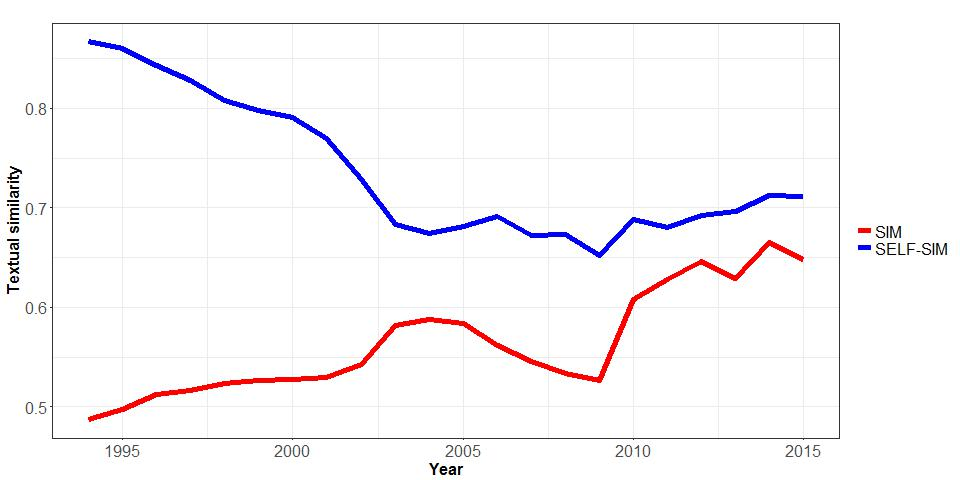
\includegraphics[width=6in, height=3in]{../figures/cossim-year}
\vspace{10mm}
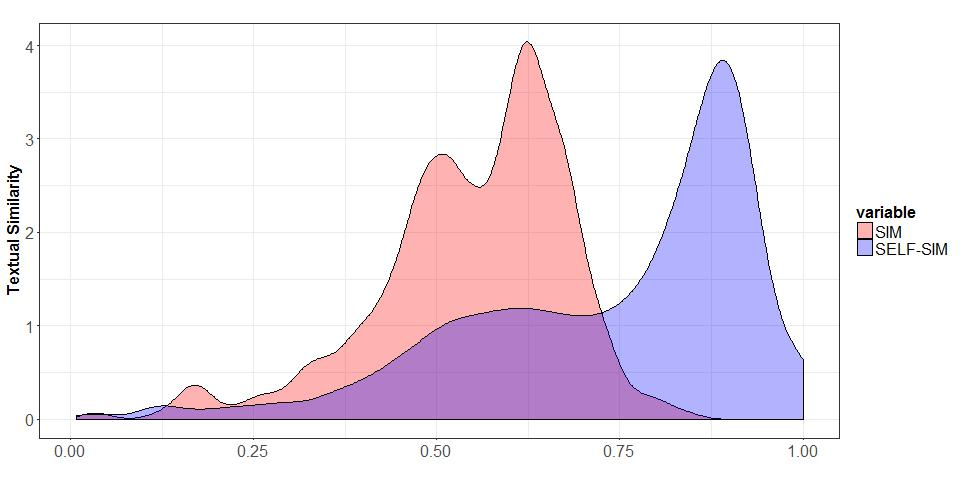
\includegraphics[width=6in, height=3in]{../figures/cossim-dist}
\captionsetup{justification=centering, width=.95\textwidth} 
\caption{\footnotesize (Top panel) Time series trends of accounting comparability measure $COMP$. (Bottom panel) Pooled cross-sectional distribution of $COMP$.} \label{cossim-figures}
\end{figure} 
\newpage
%\begin{table}[htbp]
\begin{table}[H]
\footnotesize
\centering
  \caption{\textbf{Instutional Ownership by Market Value of Equity}}
  \caption*{\footnotesize
  This table reports information on aggregate institutional holdings across different firm size (market value of equity) groups. Data span all stocks listed on the NYSE, NASDAQ, or American Stock Exchange (AMEX) and all industries over the years 1980 to 2015. Institutional ownership, $IO$, for each firm in each year as the ratio of shares held by institutions to the total shares outstanding. All variables are aggregated at the industry (two-digit SIC) level. December fiscal-year-end firms. 1980-1996 included for comparison to \cite{grinsteinmichaely2005}.
  }
\begin{tabular}{lrrrrrrr}
    \toprule
          & \multicolumn{3}{c}{Full Sample} &       & \multicolumn{3}{c}{1980 - 1996 Sample} \\
    \cmidrule{2-4} \cmidrule{6-8}
\multicolumn{1}{L{2cm}}{Market Cap Quintile} & \multicolumn{1}{C{2cm}}{Mean Market Cap (\$M)}& Obs   & \multicolumn{1}{C{2cm}}{Mean Institutional Holdings (\%) }& \multicolumn{1}{c}{} & \multicolumn{1}{C{2cm}}{Mean Market Cap (\$M)} & Obs   & \multicolumn{1}{C{2cm}}{Mean Institutional Holdings (\%)} \\ 
\hline
    \multicolumn{1}{c}{1} & 3.5   & 6,146 & 17.17 & \multicolumn{1}{c}{} & 2.6   & 2,364 & 14.64 \\
    \multicolumn{1}{c}{2} & 12.2  & 6,159 & 30.40 & \multicolumn{1}{c}{} & 8.9   & 2,371 & 24.87 \\
    \multicolumn{1}{c}{3} & 36.3  & 6,160 & 44.89 & \multicolumn{1}{c}{} & 27.3  & 2,374 & 34.41 \\
    \multicolumn{1}{c}{4} & 113.2 & 6,159 & 53.95 & \multicolumn{1}{c}{} & 88.7  & 2,371 & 42.70 \\
    \multicolumn{1}{c}{5} & 1,343.1 & 6,151 & 58.66 & \multicolumn{1}{c}{} & 689.5 & 2,368 & 49.75\\
    \multicolumn{1}{c}{All} & 3,014.8 & 30,775 & 41.02 & \multicolumn{1}{c}{} & 163.3 & 11,848 & 33.28 \\    \bottomrule
    \end{tabular} 
  \label{ior-mve-summary}
\end{table}%
 
\newpage 
\begin{sidewaystable}[H]																				
\footnotesize																			
  \centering																				
\captionsetup{width=.95\textwidth}																
 \caption[\textbf{Descriptive Statistics}]{\textbf{Descriptive Statistics}\\
\footnotesize This table presents descriptive statistics on the textual similarity of firms accounting policy disclosures, institutional ownership, and other firm characteristics. 
Institutional ownership is measured as the ratio of active-to-passive dollars invested (investors), $PCT\text{-}ACTIVE$ ($NUM\text{-}ACTIVE$)
$SIM$ denotes the aggregate mean similarity level for each firm in a specific year. 
All other variables are defined in Appendix A.}\label{summary-stats}																																
    \begin{tabular}{rrrrrrrrrr}																				
    \toprule
	\toprule																				
          &       &       & \multicolumn{7}{c}{Percentile} \\																				
    \cmidrule{4-10}																				
    \multicolumn{1}{c}{Variable} & \multicolumn{1}{c}{Mean} & \multicolumn{1}{c}{Std Dev} & \multicolumn{1}{c}{1st} & \multicolumn{1}{c}{5th} & \multicolumn{1}{c}{25th} & \multicolumn{1}{c}{50th} & \multicolumn{1}{c}{75th} & \multicolumn{1}{c}{95th} & \multicolumn{1}{c}{99th} \\ \hline																				
\multicolumn{1}{l}	{AGE}	&	15.744	&	13.452	&	0.999	&	2.001	&	5.999	&	11.001	&	21.999	&	45.254	&	58.001	\\
\multicolumn{1}{l}	{ASSETS}	&	8,334.100	&	73,577.254	&	5.381	&	15.397	&	96.843	&	455.665	&	2,235.352	&	21,873.966	&	121,274.220	\\
\multicolumn{1}{l}	{BASPREAD}	&	0.014	&	0.045	&	0.000	&	0.000	&	0.000	&	0.000	&	0.000	&	0.088	&	0.200	\\
\multicolumn{1}{l}	{RETURN}	&	0.198	&	0.817	&	-0.815	&	-0.601	&	-0.176	&	0.093	&	0.380	&	1.250	&	3.042	\\
\multicolumn{1}{l}	{DIV}	&	2.427	&	15.400	&	0.000	&	0.000	&	0.000	&	0.000	&	0.684	&	8.624	&	44.298	\\
\multicolumn{1}{l}	{LEVERAGE}	&	0.221	&	0.199	&	0.000	&	0.000	&	0.045	&	0.182	&	0.349	&	0.604	&	0.785	\\
\multicolumn{1}{l}	{MVE}	&	3,307.920	&	15,054.958	&	3.427	&	10.499	&	65.022	&	284.206	&	1,284.152	&	12,719.206	&	61,645.644	\\
\multicolumn{1}{l}	{NANALYSTS}	&	5.312	&	6.845	&	0.000	&	0.000	&	0.000	&	3.000	&	7.000	&	20.000	&	30.000	\\
\multicolumn{1}{l}	{PE}	&	30.746	&	207.525	&	-139.094	&	-15.848	&	8.328	&	16.221	&	31.366	&	116.386	&	405.000	\\
\multicolumn{1}{l}	{PRICE}	&	23.358	&	57.695	&	0.829	&	1.969	&	7.548	&	16.240	&	29.033	&	59.986	&	106.049	\\
\multicolumn{1}{l}	{Q}	&	1.504	&	3.056	&	0.103	&	0.191	&	0.623	&	0.974	&	1.598	&	4.250	&	8.951	\\
\multicolumn{1}{l}	{ROA}	&	-0.001	&	0.344	&	-0.812	&	-0.298	&	-0.003	&	0.023	&	0.061	&	0.146	&	0.267	\\
\multicolumn{1}{l}	{SP500}	&	0.112	&	0.316	&	0.000	&	0.000	&	0.000	&	0.000	&	0.000	&	1.000	&	1.000	\\
\multicolumn{1}{l}	{TANG}	&	0.518	&	0.167	&	0.061	&	0.214	&	0.434	&	0.530	&	0.606	&	0.807	&	0.927	\\
\multicolumn{1}{l}	{TURNOVER}	&	1.322	&	9.723	&	0.023	&	0.079	&	0.304	&	0.684	&	1.429	&	3.850	&	8.634	\\
\hline
\multicolumn{1}{l}	{$SIM$}	&	0.74	&	0.07	&	0.48	&	0.62	&	0.71	&	0.75	&	0.79	&	0.82	&	0.83	\\
\multicolumn{1}{l}	{$PCT\text{-}ACTIVE$}  & 0.850	&	0.140	&	0.342	&	0.609	&	0.786	&	0.868	&	0.959	&	1.000	& 1.000 \\
\multicolumn{1}{l}	{$NUM\text{-}ACTIVE$}  & 0.798	&	0.136	&	0.444	&	0.561	&	0.714	&	0.804	&	0.871	&	1.000	& 1.000 \\
    \bottomrule																				
    \end{tabular}																				
\end{sidewaystable}																				
 
\newpage
% latex table generated in R 3.2.3 by xtable 1.8-0 package
% Thu Oct 13 23:54:06 2016
\begin{table}[H]
\footnotesize
\centering
\captionsetup{width=.95\textwidth}																
 \caption{\textbf{Univariate Determinants of Accounting Comparability}}  								
 \label{cossim-uni}																				
\caption*{\footnotesize This table presents univariate regression results of $SIM$ on firm characteristics. $SIM_{t-1}$ indicates the one-year lag of similarity. All other variables are as defined in Appendix A.}
\begin{tabular}{lrrrr}
  \hline
 & Coefficient & Std Error & \emph{t} & $R^2$\\ 
  \hline
AGE & 0.0001 & 0.0001 & 2.0500 & 0.0200 \\ 
AT & 0.0029 & 0.0005 & 6.0800 & 0.1600 \\ 
BASPREAD & -0.3274 & 0.0514 & -6.3700 & 0.1700 \\ 
BHR & 0.0005 & 0.0013 & 0.3700 & 0.0000 \\ 
DIV & -0.0002 & 0.0002 & -0.8900 & 0.0000 \\ 
LEVERAGE & -0.0069 & 0.0046 & -1.4900 & 0.0100 \\ 
MVE & 0.0030 & 0.0005 & 6.3800 & 0.1700 \\ 
NANALYSTS & -0.0001 & 0.0001 & -0.8300 & 0.0000 \\ 
PE & -0.0000 & 0.0000 & -2.4000 & 0.0200 \\ 
PRICE & 0.0000 & 0.0000 & 0.8900 & 0.0000 \\ 
Q & -0.0008 & 0.0006 & -1.4300 & 0.0100 \\ 
ROA & -0.0083 & 0.0056 & -1.4900 & 0.0100 \\ 
SP500 & -0.0131 & 0.0024 & -5.5100 & 0.1300 \\ 
TANG & -0.0092 & 0.0050 & -1.8500 & 0.0100 \\ 
TURNOVER & 0.0012 & 0.0001 & 10.4800 & 0.4600 \\ 
$SIM_{t-1}$ & 0.6492 & 0.0058 & 111.7300 & 38.3300 \\
   \hline
\end{tabular}
\end{table}

\newpage
\begin{sidewaystable}[H]
\tiny
\centering
\captionsetup{width=.95\textwidth}		
\caption[\textbf{Correlation Matrix}]{\footnotesize \textbf{Correlation Matrix}\\
 This table presents a correlation matrix of institutional ownership and other firm characteristics. 
Institutional ownership is measured as the ratio of active-to-passive dollars invested (investors), $PCT\text{-}ACTIVE$ ($NUM\text{-}ACTIVE$) All other variables are defined in Appendix A.
\\
Labels are:(1) $AGE$; (2) $AT$; (3) $BASPREAD$; (4) $BHR$; (5) $DIV$; (6) $LEVERAGE$; (7) $MVE$; (8) $NANALYSTS$; (9) $PE$; (10) $PRICE$; (11) $Q$; (12) $ROA$; (13) $SP500$; (14) $TANG$; (15) $TURNOVER$; (16) $IO$; (17) $PCT-ACTIVE$; (18) $NUM\text{-}INSTITUTIONS$; (19) $NUM\text{-}ACTIVE$.}\label{corr}
\begin{tabular}{rlllllllllllllllllll}
  \hline
 & (1) & (2) & (3) & (4) & (5) & (6) & (7) & (8) & (9) & (10) & (11) & (12) & (13) & (14) & (15) & (16) & (17) & (18) & (19) \\ 
  \hline
(1) & 1 &  &  &  &  &  &  &  &  &  &  &  &  &  &  &  &  &  &  \\ 
  (2) & 0.38 & 1 &  &  &  &  &  &  &  &  &  &  &  &  &  &  &  &  &  \\ 
  (3) & -0.18 & -0.387 & 1 &  &  &  &  &  &  &  &  &  &  &  &  &  &  &  &  \\ 
  (4) & 0.072 & 0.088 & -0.011 & 1 &  &  &  &  &  &  &  &  &  &  &  &  &  &  &  \\ 
  (5) & 0.366 & 0.575 & -0.16 & 0.054 & 1 &  &  &  &  &  &  &  &  &  &  &  &  &  &  \\ 
  (6) & 0.127 & 0.28 & -0.036 & -0.03 & 0.178 & 1 &  &  &  &  &  &  &  &  &  &  &  &  &  \\ 
  (7) & 0.342 & 0.829 & -0.529 & 0.208 & 0.478 & 0.12 & 1 &  &  &  &  &  &  &  &  &  &  &  &  \\ 
  (8) & 0.312 & 0.588 & -0.48 & 0.016 & 0.296 & 0.079 & 0.692 & 1 &  &  &  &  &  &  &  &  &  &  &  \\ 
  (9) & 0.09 & 0.126 & -0.007 & 0.339 & 0.101 & -0.063 & 0.267 & 0.147 & 1 &  &  &  &  &  &  &  &  &  &  \\ 
  (10) & 0.312 & 0.629 & -0.274 & 0.18 & 0.484 & 0.051 & 0.724 & 0.5 & 0.395 & 1 &  &  &  &  &  &  &  &  &  \\ 
  (11) & -0.096 & -0.26 & -0.233 & 0.199 & -0.174 & -0.054 & 0.239 & 0.149 & 0.205 & 0.117 & 1 &  &  &  &  &  &  &  &  \\ 
  (12) & 0.143 & 0.088 & -0.063 & 0.246 & 0.228 & -0.086 & 0.275 & 0.163 & 0.379 & 0.409 & 0.305 & 1 &  &  &  &  &  &  &  \\ 
  (13) & 0.386 & 0.438 & -0.171 & 0.032 & 0.374 & 0.099 & 0.454 & 0.459 & 0.116 & 0.371 & 0.02 & 0.139 & 1 &  &  &  &  &  &  \\ 
  (14) & -0.209 & -0.376 & 0.114 & -0.003 & -0.215 & -0.363 & -0.275 & -0.165 & -0.071 & -0.198 & 0.134 & -0.033 & -0.177 & 1 &  &  &  &  &  \\ 
  (15) & -0.034 & 0.179 & -0.425 & -0.003 & -0.097 & 0.011 & 0.366 & 0.372 & -0.061 & 0.116 & 0.323 & -0.014 & 0.08 & -0.005 & 1 &  &  &  &  \\ 
  (16) & 0.304 & 0.549 & -0.47 & 0.047 & 0.192 & 0.072 & 0.667 & 0.596 & 0.144 & 0.478 & 0.167 & 0.156 & 0.268 & -0.22 & 0.494 & 1 &  &  &  \\ 
  (17) & -0.222 & -0.227 & 0.13 & -0.004 & -0.265 & -0.047 & -0.189 & -0.212 & -0.083 & -0.244 & 0.067 & -0.079 & -0.224 & 0.075 & 0.08 & -0.069 & 1 &  &  \\ 
  (18) & 0.436 & 0.731 & -0.577 & 0.064 & 0.381 & 0.115 & 0.867 & 0.763 & 0.173 & 0.596 & 0.191 & 0.194 & 0.485 & -0.268 & 0.459 & 0.795 & -0.17 & 1 &  \\ 
  (19) & -0.084 & 0.051 & -0.021 & 0.032 & -0.124 & -0.014 & 0.132 & 0.054 & -0.035 & -0.007 & 0.127 & 0.012 & -0.046 & -0.031 & 0.323 & 0.198 & 0.682 & 0.209 & 1 \\ 
   \hline
\end{tabular}
\end{sidewaystable}
 
\newpage
\centering 
\footnotesize 
\begin{longtable}{@{\extracolsep{5pt}}lD{.}{.}{-4} D{.}{.}{-4} D{.}{.}{-4} D{.}{.}{-4} } 
\caption[\textbf{Active and Passive Institutional Ownership, Regression in Levels}]{\textbf{Active and Passive Institutional Ownership, Regression in Levels}\\
\footnotesize OLS results of regressing the ratio of active-to-passive dollars invested (investors), $PCT\text{-}ACTIVE$ ($NUM\text{-}ACTIVE$) on the textual similarity of accounting policy disclosures from the ``Summary of Significant Accounting Policies'' section, $SIM$, from firms' 10-K's. Control variables are included. All other variables are defined in Appendix A.}\label{tab:levels} 
\\[-1.8ex]\hline 
\hline \\[-1.8ex] 
 & \multicolumn{4}{c}{\textit{Dependent variable:}} \\ 
\cline{2-5} 
& \multicolumn{2}{c}{$PCT\text{-}ACTIVE_{t+1}$} & \multicolumn{2}{c}{$NUM\text{-}ACTIVE_{t+1}$} \\ 
[-1.8ex] & \multicolumn{1}{c}{(1)} & \multicolumn{1}{c}{(2)} & \multicolumn{1}{c}{(3)} & \multicolumn{1}{c}{(4)}\\ 
\hline \\[-1.8ex] 
  CONSTANT & 0.2325^{***} & 0.2011^{***} & 0.0782^{***} & 0.0397^{***} \\ 
  & (0.0114) & (0.0171) & (0.0110) & (0.0147) \\ 
 PCT-ACTIVE & 0.7563^{***} & 0.7806^{***} &  &  \\ 
  & (0.0128) & (0.0155) &  &  \\ 
  NUM-ACTIVE &  &  & 0.9366^{***} & 0.9015^{***} \\ 
  &  &  & (0.0136) & (0.0178) \\ 
  SIM & -0.005^{***} & -0.0073^{***} & -0.012^{***} & -0.007^{***} \\ 
  & (0.0006) & (0.0006) & (0.0006) & (0.0006) \\ 
  MVE &  & -0.0062 &  & -0.0041 \\ 
  &  & (0.0047) &  & (0.0042) \\ 
  PRICE &  & 0.0005^{***} &  & 0.0002^{**} \\ 
  &  & (0.0001) &  & (0.0001) \\ 
  TURNOVER &  & 0.0026^{*} &  & -0.0008 \\ 
  &  & (0.0013) &  & (0.0012) \\ 
  AGE &  & 0.0003^{**} &  & 0.0003^{**} \\ 
  &  & (0.0001) &  & (0.0001) \\ 
  BASPREAD &  & 0.1134 &  & -0.1213 \\ 
  &  & (0.1510) &  & (0.1358) \\ 
  SP500 &  & -0.0153^{**} &  & -0.0134^{**} \\ 
  &  & (0.0060) &  & (0.0054) \\ 
  DIV &  & 0.0008^{**} &  & -0.0004 \\ 
  &  & (0.0003) &  & (0.0003) \\ 
  LEVERAGE &  & -0.0397^{***} &  & -0.0294^{***} \\ 
  &  & (0.0120) &  & (0.0108) \\ 
  Q &  & -0.0011 &  & 0.0044^{**} \\ 
  &  & (0.0024) &  & (0.0022) \\ 
  RETURN &  & 0.0121^{***} &  & 0.0205^{***} \\ 
  &  & (0.0035) &  & (0.0031) \\ 
  ROA &  & -0.0104 &  & -0.0311^{**} \\ 
  &  & (0.0170) &  & (0.0152) \\ 
  ASSETS &  & 0.0062 &  & 0.0132^{***} \\ 
  &  & (0.0046) &  & (0.0041) \\ 
  NANALYSTS &  & 0.0030 &  & 0.0018 \\ 
  &  & (0.0038) &  & (0.0034) \\ 
  PE &  & -0.0001^{***} &  & -0.0001 \\ 
  &  & (0.00004) &  & (0.00004) \\ 
 \hline \\[-1.8ex] 
Observations & \multicolumn{1}{c}{32,940} & \multicolumn{1}{c}{32,387} & \multicolumn{1}{c}{32,940} & \multicolumn{1}{c}{32,387} \\ 
R$^{2}$ & \multicolumn{1}{c}{0.5462} & \multicolumn{1}{c}{0.5637} & \multicolumn{1}{c}{0.6187} & \multicolumn{1}{c}{0.6484} \\ 
Adjusted R$^{2}$ & \multicolumn{1}{c}{0.5459} & \multicolumn{1}{c}{0.5607} & \multicolumn{1}{c}{0.6185} & \multicolumn{1}{c}{0.6460} \\ 
\hline 
\hline \\[-1.8ex] 
\textit{Note:}  & \multicolumn{4}{r}{$^{*}$p$<$0.1; $^{**}$p$<$0.05; $^{***}$p$<$0.01} \\ 
 & \multicolumn{4}{r}{Year and firm fixed effects included.} \\ 
 & \multicolumn{4}{r}{Standard errors are clustered at the firm level.}
\end{longtable}
 \newpage 
\centering 
  \footnotesize 
\begin{longtable}{@{\extracolsep{5pt}}lD{.}{.}{-4} D{.}{.}{-4} D{.}{.}{-4} D{.}{.}{-4} } 
\caption[\textbf{Active-to-Passive Institutional Ownership Ratio, Regression in Changes}]{\textbf{Active-to-Passive Institutional Ownership Ratio, Regression in Changes}\\
\footnotesize
OLS results of regressing changes in the ratio of active-to-passive dollars invested (investors), $PCT\text{-}ACTIVE$ ($NUM\text{-}ACTIVE$) on the textual similarity of accounting policy disclosures from the ``Summary of Significant Accounting Policies'' section, $SIM$, from firms' 10-K's. Control variables are included. All other variables are defined in Appendix A.} \label{changes} 
\\[-1.8ex]\hline 
\hline
 & \multicolumn{4}{c}{\textit{Dependent variable:}} \\ 
\cline{2-5} 
& \multicolumn{2}{c}{$\Delta PCT\text{-}ACTIVE$} & \multicolumn{2}{c}{$\Delta NUM\text{-}ACTIVE$} \\ 
[-1.8ex] & \multicolumn{1}{c}{(1)} & \multicolumn{1}{c}{(2)} & \multicolumn{1}{c}{(3)} & \multicolumn{1}{c}{(4)}\\ 
\hline \\[-1.8ex] 
CONSTANT & 0.0351^{***} & 0.0288^{***} & 0.0451^{***} & 0.0319^{***} \\ 
  & (0.0033) & (0.0034) & (0.0029) & (0.0029) \\ 
 $\Delta$SIM & -0.0018^{***} & -0.005^{***} & -0.0030^{***} & -0.0013^{**} \\ 
  & (0.0006) & (0.0006) & (0.0006) & (0.0005) \\ 
  $\Delta$MVE &  & 0.0025 &  & 0.0319^{***} \\ 
  &  & (0.0063) &  & (0.0053) \\ 
  $\Delta$PRICE &  & 0.0007^{***} &  & 0.0005^{***} \\ 
  &  & (0.0001) &  & (0.0001) \\ 
  $\Delta$TURNOVER &  & 0.0035^{***} &  & 0.0054^{***} \\ 
  &  & (0.0013) &  & (0.0011) \\ 
  $\Delta$BASPREAD &  & -0.4683^{***} &  & -0.4413^{***} \\ 
  &  & (0.1543) &  & (0.1292) \\ 
  $\Delta$DIV &  & 0.0002 &  & 0.0001 \\ 
  &  & (0.0001) &  & (0.0001) \\ 
  $\Delta$LEVERAGE &  & 0.0954^{***} &  & 0.0276 \\ 
  &  & (0.0216) &  & (0.0181) \\ 
  $\Delta$Q &  & -0.0021 &  & -0.0052^{**} \\ 
  &  & (0.0026) &  & (0.0022) \\ 
  $\Delta$RETURN &  & -0.0032 &  & -0.0120^{***} \\ 
  &  & (0.0022) &  & (0.0018) \\ 
  $\Delta$ROA &  & -0.0011 &  & 0.0120 \\ 
  &  & (0.0140) &  & (0.0118) \\ 
  $\Delta$ASSETS &  & -0.0067 &  & 0.0103 \\ 
  &  & (0.0079) &  & (0.0066) \\ 
  $\Delta$NANALYSTS &  & -0.0010 &  & -0.0007 \\ 
  &  & (0.0007) &  & (0.0005) \\ 
  $\Delta$PE &  & 0.00002 &  & 0.00003^{*} \\ 
  &  & (0.00002) &  & (0.00001) \\ 
 \hline \\[-1.8ex] 
Observations & \multicolumn{1}{c}{32,938} & \multicolumn{1}{c}{32,141} & \multicolumn{1}{c}{32,938} & \multicolumn{1}{c}{32,141} \\ 
R$^{2}$ & \multicolumn{1}{c}{0.0027} & \multicolumn{1}{c}{0.0361} & \multicolumn{1}{c}{0.0098} & \multicolumn{1}{c}{0.1154} \\ 
Adjusted R$^{2}$ & \multicolumn{1}{c}{0.0024} & \multicolumn{1}{c}{0.0302} & \multicolumn{1}{c}{0.0094} & \multicolumn{1}{c}{0.1100} \\ 
\hline 
\hline \\[-1.8ex] 
\textit{Note:}  & \multicolumn{4}{r}{$^{*}$p$<$0.1; $^{**}$p$<$0.05; $^{***}$p$<$0.01} \\ 
 & \multicolumn{4}{r}{Year and firm fixed effects included.} \\ 
 & \multicolumn{4}{r}{Standard errors are clustered at the firm level.} \\ 
\end{longtable} 

\newpage 
\begin{figure}[H] 
\centering
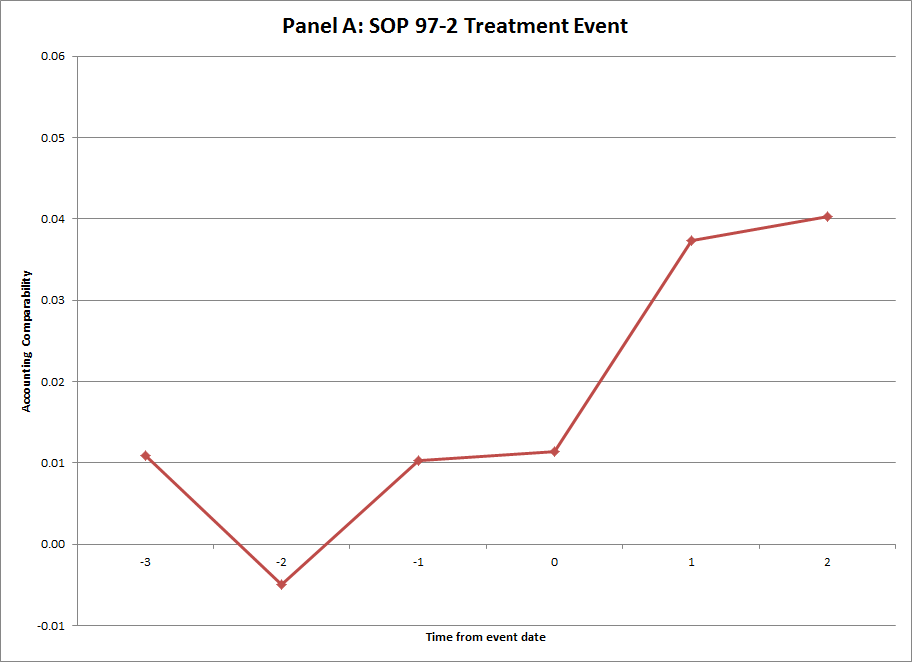
\includegraphics[width=6in, height=3in]{../figures/cossim-sop972-trends}
\vspace{10mm}
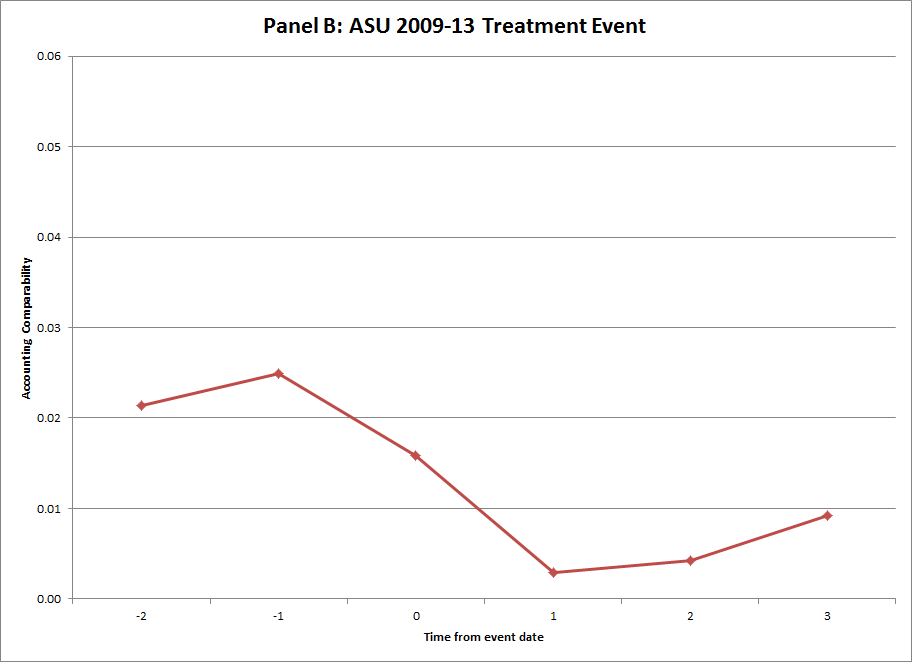
\includegraphics[width=6in, height=3in]{../figures/cossim-asu200913-trends}
\captionsetup{justification=centering, width=.95\textwidth} 
\caption{\footnotesize Trends of accounting comparability in the treatment sample net of control sample. Panel A shows the trend surrounding the SOP 97-2 event window. Panel B shows the trend surrounding the ASU 2009-13 event window.} \label{cossim-trends}
\end{figure} 
\newpage 
\centering 
\footnotesize 
\begin{longtable}{@{\extracolsep{5pt}}lD{.}{.}{-4} D{.}{.}{-4} D{.}{.}{-4} D{.}{.}{-4} } 
\caption[\textbf{Textual Similarity of Accounting Policy Disclosures Difference-in-Differences Analyses}]{\textbf{Textual Similarity of Accounting Policy Disclosures Difference-in-Differences Analyses} \\
\footnotesize Difference-in-Difference estimation of the textual similarity of accounting policy disclosures from the ``Summary of Significant Accounting Policies'' section, $SIM$, around events SOP 97-2 (dfrst and second columns) and ASU 2009-13 (third and fourth columns) event years ($TREATED$ observations). Control variables are included. All other variables are defined in Appendix A.
} \label{comp-dd} 
\\[-1.8ex]\hline 
 & \multicolumn{1}{c}{(1)} & \multicolumn{1}{c}{(2)} & \multicolumn{1}{c}{(3)} & \multicolumn{1}{c}{(4)}\\ 
\hline \\[-1.8ex] 
  CONSTANT & 0.4003^{***} & 0.4332^{***} & 0.4309^{***} & 0.4360^{***} \\ 
  & (0.0019) & (0.0107) & (0.0018) & (0.0103) \\ 
 POST\textasteriskcentered TREATED & 0.0256^{**} & 0.069^{***} & -0.0232^{**} & -0.0497^{***} \\ 
  & (0.0125) & (0.0143) & (0.0120) & (0.0130) \\ 
  TREATED & -0.0123^{**} & -0.0101 & -0.0226^{***} & -0.0157^{**} \\ 
  & (0.0059) & (0.0070) & (0.0058) & (0.0070) \\ 
  POST & 0.0562^{***} & 0.0468^{***} & -0.0797^{***} & -0.0775^{***} \\ 
  & (0.0039) & (0.0048) & (0.0038) & (0.0044) \\ 
  MVE &  & 0.000000 &  & 0.000000 \\ 
  &  & (0.000000) &  & (0.000000) \\ 
  PRICE &  & -0.00004 &  & 0.0001 \\ 
  &  & (0.0001) &  & (0.0001) \\ 
  TURNOVER &  & -0.0096^{***} &  & -0.0090^{***} \\ 
  &  & (0.0014) &  & (0.0014) \\ 
  AGE &  & -0.0002^{*} &  & -0.0003^{**} \\ 
  &  & (0.0001) &  & (0.0001) \\ 
  BASPREAD &  & -0.0084 &  & -0.0442 \\ 
  &  & (0.1405) &  & (0.1366) \\ 
  SP500 &  & 0.0418^{***} &  & 0.0321^{***} \\ 
  &  & (0.0061) &  & (0.0060) \\ 
  DIV &  & 0.0001 &  & 0.0001 \\ 
  &  & (0.0001) &  & (0.0001) \\ 
  LEVERAGE &  & 0.0339^{***} &  & 0.0343^{***} \\ 
  &  & (0.0100) &  & (0.0097) \\ 
  Q &  & 0.0030^{*} &  & 0.0040^{**} \\ 
  &  & (0.0017) &  & (0.0017) \\ 
  RETURN &  & -0.0045 &  & -0.0020 \\ 
  &  & (0.0033) &  & (0.0032) \\ 
  ROA &  & 0.0525^{***} &  & 0.0379^{**} \\ 
  &  & (0.0151) &  & (0.0147) \\ 
  ASSETS &  & -0.0058^{***} &  & -0.0034^{*} \\ 
  &  & (0.0018) &  & (0.0018) \\ 
  NANALYSTS &  & 0.0028 &  & 0.0067^{**} \\ 
  &  & (0.0035) &  & (0.0034) \\ 
  PE &  & 0.00005^{**} &  & 0.00002 \\ 
  &  & (0.00002) &  & (0.00002) \\ 
 \hline \\[-1.8ex] 
Observations & \multicolumn{1}{c}{4,655} & \multicolumn{1}{c}{3,655} & \multicolumn{1}{c}{4,655} & \multicolumn{1}{c}{3,655} \\ 
R$^{2}$ & \multicolumn{1}{c}{0.0468} & \multicolumn{1}{c}{0.0790} & \multicolumn{1}{c}{0.0908} & \multicolumn{1}{c}{0.1292} \\ 
Adjusted R$^{2}$ & \multicolumn{1}{c}{0.0462} & \multicolumn{1}{c}{0.0747} & \multicolumn{1}{c}{0.0902} & \multicolumn{1}{c}{0.1251} \\ 
\hline 
\hline \\[-1.8ex] 
\textit{Note:}  & \multicolumn{4}{r}{$^{*}$p$<$0.1; $^{**}$p$<$0.05; $^{***}$p$<$0.01} \\ 
\end{longtable} 
\newpage 
\begin{figure}[H] 
\centering
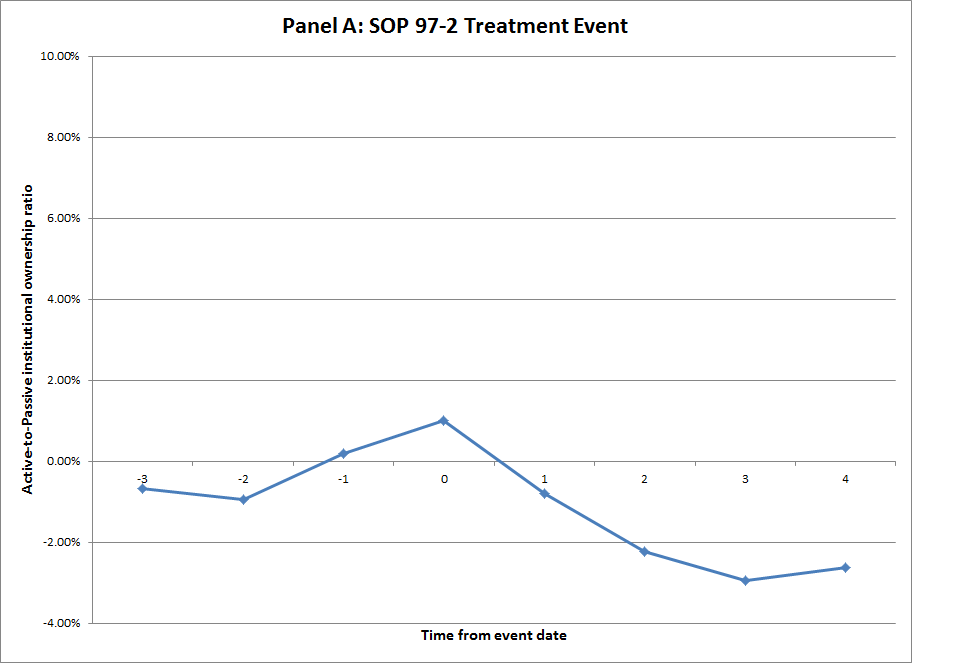
\includegraphics[width=6in, height=3in]{../figures/sop972-trends}
\vspace{10mm}
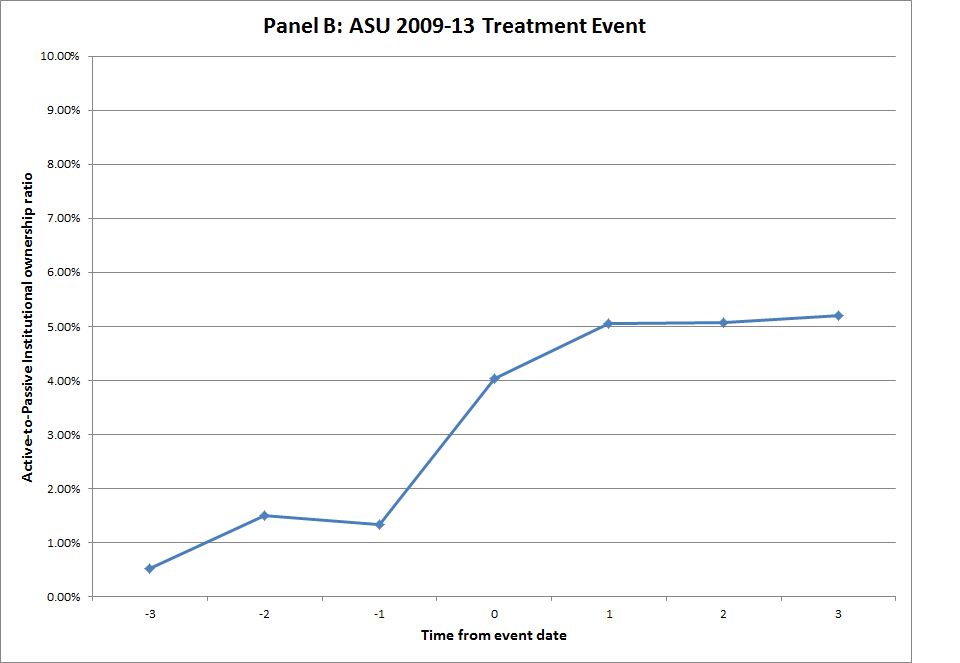
\includegraphics[width=6in, height=3in]{../figures/asu200913-trends}
\captionsetup{justification=centering, width=.95\textwidth} 
\caption{\footnotesize Trends of active-to-passive institutional investor ownership in the treatment sample net of control sample. Panel A shows the trend surrounding the SOP 97-2 event window. Panel B shows the trend surrounding the ASU 2009-13 event window.} \label{trends}
\end{figure} 
\newpage

\centering
\begin{longtable}{lrrrr} 
\caption[\textbf{Post-match differences in pre-period for DD}]{\textbf{Post-match differences in pre-period for DD}\\
\footnotesize This table reports diagnostics of the DD tests of how exogeneous shocks to comparability (SOP 97-2 and ASU 2009-13) afffect the ratio of active-to-passive institutional investor ownership in firms. For the SOP 97-2 event, the sample begins with all firm-years from 1995 to 2001 with non-missing matching variables and outcome variables during a six-year window around the event year. For the ASU 2009-13 event, the sample begins with all firm-years from 2008 to 2013 with non-missing matching variables and outcome variables during a five-year window around the event year. Treatment firms are those likely to engange in multi-element contracts for software products and services. The benchmark control firms are found by matching treatment firms to candidate control firms on firm-level variables.}\label{post-match} \\
  \hline
  \hline
  Panel A: SOP 97-2 treatment.\\
  \hline
  \endfirsthead
 & Treatment & Control & Differences & $t$-statistic \\ 
  \hline
  \endhead
  $PCT\text{-}ACTIVE$ & 0.816 & 0.818 & -0.002 & -0.261 \\
  $NUM\text{-}ACTIVE$ & 0.753 & 0.747 & 0.006 & 1.357 \\
  $COMP$ & 0.472 & 0.455 & 0.017 & 1.241\\
AGE & 7.05 & 7.26 & -0.22 & -0.49 \\ 
  ASSETS & 4.66 & 4.68 & -0.03 & -0.38 \\ 
  BASPREAD & 0.00 & 0.01 & -0.00 & -0.23 \\ 
  RETURN & 0.16 & 0.16 & -0.00 & -0.07 \\ 
  DIV & 0.28 & 0.24 & 0.04 & 0.50 \\ 
  LEVERAGE & 0.08 & 0.08 & -0.00 & -0.02 \\ 
  MVE & 5.47 & 5.47 & -0.00 & -0.07 \\ 
  NANALYSTS & 4.63 & 4.58 & 0.05 & 0.18 \\ 
  PE & 53.98 & 37.83 & 16.15 & 3.06 \\ 
  PRICE & 20.02 & 19.32 & 0.70 & 0.88 \\ 
  Q & 3.11 & 2.97 & 0.13 & 1.11 \\ 
  ROA & -0.02 & -0.05 & 0.03 & 2.35 \\ 
  SP500 & 0.04 & 0.03 & 0.01 & 1.03 \\ 
  TURNOVER & 1.91 & 1.79 & 0.12 & 1.34 \\ 
   \hline \\
   Panel B: ASU 2009-13 treatment.\\
   \hline
 & Treatment & Control & Differences & $t$-statistics \\ 
  \hline
  $PCT\text{-}ACTIVE$ & 0.848 & 0.817 & 0.031 & 1.318 \\
$NUM\text{-}ACTIVE$ & 0.787 & 0.812 & -0.025 & -1.508\\
$COMP$ & 0.359 & 0.398 & -0.039 & -1.368\\
AGE & 13.20 & 13.40 & -0.20 & -0.38 \\ 
  ASSETS & 6.07 & 5.99 & 0.08 & 0.90 \\ 
  BASPREAD & 0.00 & 0.00 & -0.00 & -1.05 \\ 
  RETURN & 0.15 & 0.15 & -0.00 & -0.01 \\ 
  DIV & 1.72 & 0.95 & 0.76 & 2.34 \\ 
  LEVERAGE & 0.10 & 0.11 & -0.02 & -2.00 \\ 
  MVE & 6.12 & 6.05 & 0.07 & 0.77 \\ 
  NANALYSTS & 7.66 & 6.89 & 0.77 & 2.36 \\ 
  PE & 20.91 & 20.84 & 0.07 & 0.02 \\ 
  PRICE & 14.76 & 19.48 & -4.72 & -4.66 \\ 
  Q & 1.52 & 1.63 & -0.11 & -1.56 \\ 
  ROA & -0.02 & -0.04 & 0.01 & 1.31 \\ 
  SP500 & 0.08 & 0.06 & 0.02 & 1.57 \\ 
  TURNOVER & 2.09 & 2.19 & -0.10 & -0.90 \\ 
   \hline
\end{longtable}
 
\newpage
\centering 
\footnotesize 
\begin{longtable}{@{\extracolsep{5pt}}lD{.}{.}{-4} D{.}{.}{-4} D{.}{.}{-4} D{.}{.}{-4} } 
\caption[\textbf{Difference-in-Differences Analysis around SOP 97-3}]{\textbf{Difference-in-Differences Analysis around SOP 97-3}\\
\footnotesize
Difference-in-Difference estimation of  the ratio of active-to-passive dollars invested (investors), $PCT\text{-}ACTIVE$ ($NUM\text{-}ACTIVE$) around  SOP 97-2 event years ($TREATED$ observations). Control variables are included. All other variables are defined in Appendix A.} \label{dd1}
\\[-1.8ex]\hline 
\hline 
 & \multicolumn{4}{c}{\textit{Dependent variable:}} \\ 
\cline{2-5} 
 & \multicolumn{2}{c}{$PCT\text{-}ACTIVE_{t+1}$} & \multicolumn{2}{c}{$NUM\text{-}ACTIVE_{t+1}$} \\
[-1.8ex] & \multicolumn{1}{c}{(1)} & \multicolumn{1}{c}{(2)} & \multicolumn{1}{c}{(3)} & \multicolumn{1}{c}{(4)}\\ 
\hline \\[-1.8ex] 
CONSTANT & 0.8131^{***} & 0.8341^{***} & 0.7416^{***} & 0.6538^{***} \\ 
  & (0.0047) & (0.0122) & (0.0036) & (0.0088) \\ 
 POST \textasteriskcentered  TREATED & -0.048^{**} & -0.04^{**} & -0.027^{***} & -0.05^{***} \\ 
  & (0.0290) & (0.0189) & (0.0069) & (0.0065) \\ 
  TREATED & 0.0050 & 0.0047 & 0.0138^{***} & 0.0126^{**} \\ 
  & (0.0069) & (0.0068) & (0.0053) & (0.0050) \\ 
  POST & -0.0343^{***} & -0.0359^{***} & -0.0054 & -0.0058 \\ 
  & (0.0063) & (0.0063) & (0.0048) & (0.0046) \\ 
  MVE &  & -0.0142^{**} &  & 0.0255^{***} \\ 
  &  & (0.0064) &  & (0.0046) \\ 
  PRICE &  & 0.0001 &  & 0.0001 \\ 
  &  & (0.0002) &  & (0.0001) \\ 
  TURNOVER &  & -0.000005 &  & 0.0023^{***} \\ 
  &  & (0.0011) &  & (0.0008) \\ 
  AGE &  & -0.0019^{***} &  & -0.0024^{***} \\ 
  &  & (0.0003) &  & (0.0003) \\ 
  BASPREAD &  & 0.2447^{*} &  & 0.6080^{***} \\ 
  &  & (0.1303) &  & (0.0949) \\ 
  SP500 &  & -0.0640^{***} &  & -0.0058 \\ 
  &  & (0.0137) &  & (0.0100) \\ 
  DIV &  & -0.0004 &  & -0.0028^{***} \\ 
  &  & (0.0015) &  & (0.0011) \\ 
  LEVERAGE &  & -0.0156 &  & -0.0150 \\ 
  &  & (0.0200) &  & (0.0146) \\ 
  Q &  & 0.0007 &  & -0.0026 \\ 
  &  & (0.0022) &  & (0.0016) \\ 
  RETURN &  & 0.0102^{***} &  & -0.0059^{***} \\ 
  &  & (0.0030) &  & (0.0022) \\ 
  ROA &  & 0.0288^{***} &  & 0.0300^{***} \\ 
  &  & (0.0099) &  & (0.0072) \\ 
  ASSETS &  & 0.0097 &  & -0.0069 \\ 
  &  & (0.0065) &  & (0.0047) \\ 
  NANALYSTS &  & 0.0156^{***} &  & -0.0005 \\ 
  &  & (0.0048) &  & (0.0035) \\ 
  PE &  & 0.000001 &  & 0.000004 \\ 
  &  & (0.00002) &  & (0.00002) \\ 
 \hline \\[-1.8ex] 
Observations & \multicolumn{1}{c}{3,402} & \multicolumn{1}{c}{3,402} & \multicolumn{1}{c}{3,402} & \multicolumn{1}{c}{3,402} \\ 
R$^{2}$ & \multicolumn{1}{c}{0.0169} & \multicolumn{1}{c}{0.0556} & \multicolumn{1}{c}{0.0064} & \multicolumn{1}{c}{0.1320} \\ 
Adjusted R$^{2}$ & \multicolumn{1}{c}{0.0160} & \multicolumn{1}{c}{0.0509} & \multicolumn{1}{c}{0.0055} & \multicolumn{1}{c}{0.1277} \\ 
\hline 
\hline \\[-1.8ex] 
\textit{Note:}  & \multicolumn{4}{r}{$^{*}$p$<$0.1; $^{**}$p$<$0.05; $^{***}$p$<$0.01} \\ 
\end{longtable} 



\newpage
\centering 
\footnotesize 
\begin{longtable}{@{\extracolsep{5pt}}lD{.}{.}{-4} D{.}{.}{-4} D{.}{.}{-4} D{.}{.}{-4} } 
\caption[\textbf{Difference-in-Differences Analysis around ASU 2009-13}]{\textbf{Difference-in-Differences Analysis around ASU 2009-13}\\
\footnotesize
Difference-in-Difference estimation of  the ratio of active-to-passive dollars invested (investors), $PCT\text{-}ACTIVE$ ($NUM\text{-}ACTIVE$) around ASU 2009-13 event years ($TREATED$ observations). Control variables are included. All other variables are defined in Appendix A.} \label{dd2}
\\[-1.8ex]\hline 
\hline \\[-1.8ex] 
 & \multicolumn{4}{c}{\textit{Dependent variable:}} \\ 
\cline{2-5} 
 & \multicolumn{2}{c}{$PCT\text{-}ACTIVE_{t+1}$} & \multicolumn{2}{c}{$NUM\text{-}ACTIVE_{t+1}$} \\
[-1.8ex] & \multicolumn{1}{c}{(1)} & \multicolumn{1}{c}{(2)} & \multicolumn{1}{c}{(3)} & \multicolumn{1}{c}{(4)}\\ 
\hline \\[-1.8ex] 
CONSTANT & 0.8656^{***} & 0.8881^{***} & 0.8186^{***} & 0.7341^{***} \\ 
  & (0.0032) & (0.0097) & (0.0022) & (0.0063) \\ 
 POSTS \textasteriskcentered  TREATED & 0.0780^{***} & 0.0188^{***} & 0.0063^{*} & 0.0058^{*} \\ 
  & (0.0065) & (0.0043) & (0.0045) & (0.0040) \\ 
  TREATED & 0.0036 & 0.0054 & 0.0009 & -0.0009 \\ 
  & (0.0046) & (0.0045) & (0.0031) & (0.0029) \\ 
  POST & 0.0900^{***} & 0.0089^{**} & 0.0035 & 0.0031 \\ 
  & (0.0046) & (0.0046) & (0.0032) & (0.0030) \\ 
  MVE &  & -0.0047 &  & 0.0062^{**} \\ 
  &  & (0.0042) &  & (0.0027) \\ 
  PRICE &  & 0.0001 &  & -0.0002^{***} \\ 
  &  & (0.0001) &  & (0.0001) \\ 
  TURNOVER &  & -0.0020^{**} &  & 0.0027^{***} \\ 
  &  & (0.0009) &  & (0.0006) \\ 
  AGE &  & -0.0011^{***} &  & -0.0005^{***} \\ 
  &  & (0.0002) &  & (0.0001) \\ 
  BASPREAD &  & 0.7238^{***} &  & -0.4499^{***} \\ 
  &  & (0.2394) &  & (0.1552) \\ 
  SP500 &  & -0.0318^{***} &  & -0.0129^{***} \\ 
  &  & (0.0075) &  & (0.0049) \\ 
  DIV &  & -0.0003 &  & -0.0014^{***} \\ 
  &  & (0.0003) &  & (0.0002) \\ 
  LEVERAGE &  & -0.0031 &  & -0.0259^{***} \\ 
  &  & (0.0127) &  & (0.0082) \\ 
  Q &  & 0.0015 &  & 0.0006 \\ 
  &  & (0.0019) &  & (0.0013) \\ 
  RETURN &  & 0.0193^{***} &  & -0.0010 \\ 
  &  & (0.0024) &  & (0.0015) \\ 
  ROA &  & -0.0195^{**} &  & 0.0203^{***} \\ 
  &  & (0.0094) &  & (0.0061) \\ 
  ASSETS &  & 0.0042 &  & 0.0060^{**} \\ 
  &  & (0.0042) &  & (0.0027) \\ 
  NANALYSTS &  & -0.0036 &  & 0.0112^{***} \\ 
  &  & (0.0031) &  & (0.0020) \\ 
  PE&  & 0.00001 &  & 0.00001 \\ 
  &  & (0.00002) &  & (0.00001) \\ 
 \hline \\[-1.8ex] 
Observations & \multicolumn{1}{c}{2,550} & \multicolumn{1}{c}{2,550} & \multicolumn{1}{c}{2,550} & \multicolumn{1}{c}{2,550} \\ 
R$^{2}$ & \multicolumn{1}{c}{0.2160} & \multicolumn{1}{c}{0.2791} & \multicolumn{1}{c}{0.0774} & \multicolumn{1}{c}{0.2428} \\ 
Adjusted R$^{2}$ & \multicolumn{1}{c}{0.2151} & \multicolumn{1}{c}{0.2742} & \multicolumn{1}{c}{0.0763} & \multicolumn{1}{c}{0.2378} \\ 
\hline 
\hline \\[-1.8ex] 
\textit{Note:}  & \multicolumn{4}{r}{$^{*}$p$<$0.1; $^{**}$p$<$0.05; $^{***}$p$<$0.01} \\ 
\end{longtable}
\newpage
\centering 
\footnotesize 
\begin{longtable}{@{\extracolsep{5pt}}lD{.}{.}{-4} D{.}{.}{-4} D{.}{.}{-4} D{.}{.}{-4} } 
\caption[\textbf{Earnings Management Difference-in-Differences Analyses}]{\textbf{Earnings Management Difference-in-Differences Analyses}\\
\footnotesize Difference-in-Difference estimation of propensity to just exceed earnings expectations (a proxy for earnings management) around SOP 97-2 (frst and second columns) and ASU 2009-13 (third and fourth columns) event years ($TREATED$ observations).} \label{meet} 
\\[-1.8ex]\hline 
\cline{2-5} 
\\[-1.8ex] & \multicolumn{1}{c}{(1)} & \multicolumn{1}{c}{(2)} & \multicolumn{1}{c}{(3)} & \multicolumn{1}{c}{(4)}\\ 
\hline \\[-1.8ex] 
 POST \textasteriskcentered  TREATED & -0.0143 & -0.0181^{*} & -0.0078 & -0.0135 \\ 
  & (0.0104) & (0.0103) & (0.0134) & (0.0131) \\ 
  TREATED & 0.0240^{***} & 0.0099^{**} & 0.0225^{***} & 0.0083^{*} \\ 
  & (0.0046) & (0.0047) & (0.0044) & (0.0045) \\ 
  POST & 0.0018 & 0.0019 & -0.0289^{***} & -0.0131^{**} \\ 
  & (0.0048) & (0.0047) & (0.0059) & (0.0059) \\ 
  MVE &  & 0.000001^{**} &  & 0.000001^{**} \\ 
  &  & (0.000000) &  & (0.000000) \\ 
  PRICE &  & -0.0005^{***} &  & -0.0005^{***} \\ 
  &  & (0.0001) &  & (0.0001) \\ 
  TURNOVER &  & -0.0120^{***} &  & -0.0121^{***} \\ 
  &  & (0.0010) &  & (0.0010) \\ 
  AGE &  & -0.0002^{*} &  & -0.0002^{*} \\ 
  &  & (0.0001) &  & (0.0001) \\ 
  BASPREAD &  & -0.3521^{***} &  & -0.3578^{***} \\ 
  &  & (0.1176) &  & (0.1176) \\ 
  SP500 &  & 0.0232^{***} &  & 0.0212^{***} \\ 
  &  & (0.0056) &  & (0.0056) \\ 
  DIV &  & -0.0003 &  & -0.0003 \\ 
  &  & (0.0003) &  & (0.0003) \\ 
  LEVERAGE &  & -0.0346^{***} &  & -0.0358^{***} \\ 
  &  & (0.0094) &  & (0.0094) \\ 
  Q &  & 0.0225^{***} &  & 0.0224^{***} \\ 
  &  & (0.0013) &  & (0.0013) \\ 
  RETURN &  & 0.0083^{***} &  & 0.0086^{***} \\ 
  &  & (0.0027) &  & (0.0027) \\ 
  ROA &  & 0.1897^{***} &  & 0.1902^{***} \\ 
  &  & (0.0105) &  & (0.0105) \\ 
  AT &  & -0.0049^{***} &  & -0.0045^{***} \\ 
  &  & (0.0016) &  & (0.0016) \\ 
  NANALYSTS &  & 0.0010 &  & 0.0014 \\ 
  &  & (0.0028) &  & (0.0028) \\ 
  PE &  & 0.0006^{***} &  & 0.0006^{***} \\ 
  &  & (0.00002) &  & (0.00002) \\ 
  Constant & 0.1180^{***} & 0.1283^{***} & 0.1209^{***} & 0.1272^{***} \\ 
  & (0.0018) & (0.0084) & (0.0018) & (0.0084) \\ 
 \hline \\[-1.8ex] 
Observations & \multicolumn{1}{c}{44,595} & \multicolumn{1}{c}{44,266} & \multicolumn{1}{c}{44,595} & \multicolumn{1}{c}{44,266} \\ 
R$^{2}$ & \multicolumn{1}{c}{0.0006} & \multicolumn{1}{c}{0.0514} & \multicolumn{1}{c}{0.0013} & \multicolumn{1}{c}{0.0516} \\ 
Adjusted R$^{2}$ & \multicolumn{1}{c}{0.0006} & \multicolumn{1}{c}{0.0511} & \multicolumn{1}{c}{0.0013} & \multicolumn{1}{c}{0.0512} \\ 
\hline 
\hline \\[-1.8ex] 
\textit{Note:}  & \multicolumn{4}{r}{$^{*}$p$<$0.1; $^{**}$p$<$0.05; $^{***}$p$<$0.01} \\ 
\end{longtable} 

\newpage
\centering 
\footnotesize 
\begin{longtable}{@{\extracolsep{5pt}}lD{.}{.}{-4} D{.}{.}{-4} D{.}{.}{-4} D{.}{.}{-4} } 
  \caption[\textbf{Voluntary Disclosure Difference-in-Differences Analyses}]{\textbf{Voluntary Disclosure Difference-in-Differences Analyses}\\
  \footnotesize
Difference-in-Difference estimation of management forecasts (a proxy for voluntary disclosure) around SOP 97-2 (frst and second columns) and ASU 2009-13 (third and fourth columns) event years ($TREATED$ observations).} \label{cig-dd} 
\\[-1.8ex]\hline 
\cline{2-5} 
\\[-1.8ex] & \multicolumn{1}{c}{(1)} & \multicolumn{1}{c}{(2)} & \multicolumn{1}{c}{(3)} & \multicolumn{1}{c}{(4)}\\ 
\hline \\[-1.8ex] 
 POST \textasteriskcentered  TREATED & 0.4340^{***} & 0.2515^{*} & -0.1199 & -0.0799 \\ 
  & (0.1456) & (0.1426) & (0.2675) & (0.2545) \\ 
 TREATED & -0.6466^{***} & -0.3292^{***} & -0.5570^{***} & -0.2342^{***} \\ 
  & (0.0651) & (0.0670) & (0.0619) & (0.0644) \\ 
  POST & -2.3951^{***} & -1.9278^{***} & -0.4963^{***} & -1.2334^{***} \\ 
  & (0.0676) & (0.0671) & (0.1235) & (0.1200) \\ 
  MVE &  & 0.000004 &  & 0.000001 \\ 
  &  & (0.00001) &  & (0.00001) \\ 
  PRICE &  & 0.0046^{**} &  & 0.0055^{***} \\ 
  &  & (0.0018) &  & (0.0019) \\ 
  TURNOVER &  & 0.0308^{***} &  & 0.0409^{***} \\ 
  &  & (0.0034) &  & (0.0035) \\ 
  AGE &  & 0.0097^{***} &  & 0.0150^{***} \\ 
  &  & (0.0019) &  & (0.0019) \\ 
  BASPREAD &  & -2.3846 &  & -3.1523 \\ 
  &  & (2.3728) &  & (2.4224) \\ 
  SP500 &  & -0.2885^{***} &  & -0.4761^{***} \\ 
  &  & (0.0847) &  & (0.0864) \\ 
  DIV &  & 0.0015 &  & 0.0030 \\ 
  &  & (0.0065) &  & (0.0066) \\ 
  LEVERAGE &  & -1.0602^{***} &  & -1.6006^{***} \\ 
  &  & (0.1429) &  & (0.1451) \\ 
  Q &  & -0.0007 &  & -0.0480^{**} \\ 
  &  & (0.0234) &  & (0.0239) \\ 
  RETURN &  & 0.0492 &  & 0.0941^{**} \\ 
  &  & (0.0434) &  & (0.0443) \\ 
  ROA &  & 1.6958^{***} &  & 2.1996^{***} \\ 
  &  & (0.1769) &  & (0.1791) \\ 
  AT &  & 0.3979^{***} &  & 0.4501^{***} \\ 
  &  & (0.0281) &  & (0.0287) \\ 
  NANALYSTS &  & 0.2527^{***} &  & 0.2795^{***} \\ 
  &  & (0.0349) &  & (0.0357) \\ 
  PE &  & -0.0024^{***} &  & -0.0029^{***} \\ 
  &  & (0.0005) &  & (0.0005) \\ 
  Constant & 4.5808^{***} & 0.9701^{***} & 4.1311^{***} & 0.2570 \\ 
  & (0.0301) & (0.1572) & (0.0287) & (0.1587) \\ 
 \hline \\[-1.8ex] 
Observations & \multicolumn{1}{c}{20,710} & \multicolumn{1}{c}{20,075} & \multicolumn{1}{c}{20,710} & \multicolumn{1}{c}{20,075} \\ 
R$^{2}$ & \multicolumn{1}{c}{0.0709} & \multicolumn{1}{c}{0.1528} & \multicolumn{1}{c}{0.0053} & \multicolumn{1}{c}{0.1169} \\ 
Adjusted R$^{2}$ & \multicolumn{1}{c}{0.0708} & \multicolumn{1}{c}{0.1521} & \multicolumn{1}{c}{0.0052} & \multicolumn{1}{c}{0.1162} \\ 
\hline 
\hline \\[-1.8ex] 
\textit{Note:}  & \multicolumn{4}{r}{$^{*}$p$<$0.1; $^{**}$p$<$0.05; $^{***}$p$<$0.01}\\
\end{longtable} 

\justify
\end{document}